\documentclass[11pt]{article}
\usepackage{xeCJK}
\usepackage{geometry}
\usepackage{bm}
\usepackage{amsmath}
\usepackage{graphicx}
\usepackage{hyperref}
\usepackage{subfigure}
\usepackage{datetime}
\usepackage{fontspec}
\usepackage{fancyhdr}
\usepackage{indentfirst}
\usepackage{titlesec}
\usepackage[round]{natbib}
\usepackage{float}
\usepackage{booktabs}
\usepackage{enumitem}

% global style
\geometry{b5paper,left=0.6in,right=0.6in,top=1in,bottom=0.8in}
\linespread{1.3}
\setlength{\parindent}{2em}

\renewcommand{\today}{\small \number\year 年 \number\month 月 \number\day 日}
\renewcommand{\abstractname}{\normalsize 摘\ \ 要}
\renewcommand{\contentsname}{目录}
\renewcommand{\refname}{参考文献}
\renewcommand{\sectionmark}[1]{\markright{第\,\thesection\,章\, #1}}

% title style
\titleformat*{\section}{\Large\bfseries}
\titleformat*{\subsection}{\large\bfseries}
\titleformat*{\subsubsection}{\normalsize\bfseries}

% font style
\setCJKmainfont{SimSun}[BoldFont=SimHei, ItalicFont=KaiTi]
\setmainfont{Times New Roman}[BoldFont=Arial]

% page style
\fancypagestyle{assignment}{
    \fancyhf{}
    \fancyfoot[C]{\thepage}
    \fancyhead[L]{\small 廖紫默 (SA21005043)}
    \fancyhead[C]{\small \textbf{计算流体力学}}
    \fancyhead[R]{\small 2022年春}
    \renewcommand{\headrulewidth}{0.4pt}
    \renewcommand{\footrulewidth}{0.4pt}
}
\pagestyle{assignment}

% ref style (in chinese)
\def\equationautorefname{式}%
\def\footnoteautorefname{脚注}%
\def\itemautorefname{项}%
\def\figureautorefname{图}%
\def\figurename{图}
\def\tableautorefname{表}%
\def\tablename{表}
\def\partautorefname{篇}%
\def\appendixautorefname{附录}%
\def\chapterautorefname{章}%
\def\sectionautorefname{节}%
\def\subsectionautorefname{小节}%
\def\subsubsectionautorefname{subsubsection}%
\def\paragraphautorefname{段落}%
\def\subparagraphautorefname{子段落}%
\def\FancyVerbLineautorefname{行}%
\def\theoremautorefname{定理}%

% header
\title{\LARGE\textbf{计算流体力学 大作业报告}}
\author{\normalsize 廖紫默 (SA21005043)\\
\small 近代力学系,中国科学技术大学\\
\small \href{mailto:zimoliao@mail.ustc.edu.cn}{zimoliao@mail.ustc.edu.cn}}
\date{\today}

\begin{document}

% titlepage
\maketitle
\thispagestyle{assignment}
\pagenumbering{roman}
% \begin{abstract}
%     gp
% \end{abstract}

\tableofcontents
% titlepage end

% part 2
\newpage
\pagenumbering{arabic}
\setcounter{page}{1}
\section{Poisson equation}
求解Poisson方程并绘制等值线$\phi=\left(0.05,\ 0.2,\ 0.5,\ 0.75,\ 1\right)$:
\begin{align}
	 & \frac{\partial^2\phi}{\partial x^2}+\frac{\partial^2\phi}{\partial y^2}=\sin{x}\cos{y},\quad 0\leq x\leq 1,\ 0\leq y\leq 1, \label{eqn:poisson} \\
	 & \text{BCs: }\left\{\begin{array}{ll}
		\phi(0,y)=0,                  & \phi(1,y)=y-\dfrac{\sin{1}\cos{y}}{2}, \\[8pt]
		\phi(x,0)=-\dfrac{\sin x}{2}, & \phi(1,y)=x-\dfrac{\sin{x}\cos{1}}{2}
	\end{array}\right.
\end{align}

要求采用方法:
\begin{enumerate}[label=(\arabic*)]
	\item Jacobi、G-S选一;SOR、线SOR、块SOR选一。迭代法要求误差$10^{-6}$。
	\item CG方法、MG方法选一。
\end{enumerate}

\subsection{Discretization}
采用二阶精度的中心差分格式近似二阶导数项:
\begin{equation}
	\left(\frac{\partial^2\phi}{\partial x^2}\right)_i\simeq\frac{\phi_{i+1}+\phi_{i-1}-2\phi_i}{(\Delta x)^2}
\end{equation}
Poisson方程转化为五点离散的代数方程组:
\begin{equation}
	A_P\phi_P+A_W\phi_W+A_E\phi_E+A_S\phi_S+A_N\phi_N=Q_P
\end{equation}
其中$A_{K},\ K=(P,W,E,S,N)$为插值系数,$Q_P$为右端项。

\subsection{Explicit methods}
对于一般的线性代数方程组:
\begin{equation}
	A\bm{\phi}=\bm{Q} \label{eqn:algebra}
\end{equation}
其数值解法通常分为直接方法和迭代方法两大类。虽然前者(Gauss消去、LU分解)可以直接得到精确解(计算机精度下),但在一般的PDE问题中,离散误差远大于计算精度\citep{ferziger_computational_2020},采用低效的直接解法是不明智的选择。由此,代数方程组(特别是大型稀疏系统)的迭代求解方法在CFD中取得了广泛应用\citep{saad_iterative_2003}。

迭代方法的基本思想在于将\autoref{eqn:algebra}转化为下述迭代方程:
\begin{equation}
	M\bm{\phi}^{n+1}=N\bm{\phi}^n+\bm{B}
\end{equation}
令$A=M-N,\ \bm{B}=\bm{Q}$,那么当迭代收敛时,$\bm{\phi}^{n+1}=\bm{\phi}^n=\bm{\phi}$,上式等价于原始方程组。后续介绍的几类迭代方法,其本质区别就在于$M$、$N$采用不同的构造形式。

\subsubsection{Jacobi method}
Jacobi方法将$M$选为系数矩阵$A$的对角部分,$N$为非对角部分,迭代式中$M$的逆可以由对角元素分之一直接得到,非常容易构造与求解。离散形式的迭代方程为:
\begin{equation}
	\phi_P^{n+1}=\frac{Q_P-A_S\phi_S^n-A_W\phi_W^n-A_N\phi_N^n-A_E\phi_E^n}{A_P}
\end{equation}
若记$A=L+D+U$,分别表示其下三角、对角、上三角部分,那么Jacobi方法可以写为矩阵形式\citep{sauer_numerical_2018}:
\begin{equation}
	\bm{\phi}^{n+1}=D^{-1}\left[\bm{B}-(L+U)\bm{\phi}^n\right]
\end{equation}

\subsubsection{Gauss-Seidel (GS) method}
Gauss-Seidel方法在Jacobi方法的基础上做了细微的优化,即将每个网格点上迭代更新的值立即用于下一点的迭代。
\begin{equation}
	\phi_P^{n+1}=\frac{Q_P-A_S\phi_S^{n+1}-A_W\phi_W^{n+1}-A_N\phi_N^n-A_E\phi_E^n}{A_P}
\end{equation}
矩阵形式写为(从左下,即西南角开始迭代):
\begin{equation}
	\bm{\phi}^{n+1}=D^{-1}\left(\bm{B}-U\bm{\phi}^n-L\bm{\phi}^{n+1}\right)
\end{equation}

\subsubsection{Successive over-relaxation (SOR) method}
SOR的思路是在GS方法基础上引入超松弛因子$2>\omega>1$来加速迭代,实现快速收敛。
\begin{equation}
	\phi_P^{n+1}=\omega\frac{Q_P-A_S\phi_S^{n+1}-A_W\phi_W^{n+1}-A_N\phi_N^n-A_E\phi_E^n}{A_P}+(1-\omega)\phi_P^n
\end{equation}
对于椭圆型PDE,矩形几何,Dirichlet边界条件的情况,可选取$\omega=2/[1+\sin{(\pi/N)}]$,$N$为网格数\citep{ferziger_computational_2020,brazier_optimum_1974}。

\subsection{Semi-implicit methods}

\subsubsection{TDMA}
虽然Gauss消去与LU分解两种直接解法时间复杂度很高,前者为$\mathcal{O}(N^3)$。但在系数矩阵为三对角矩阵这一特殊情况下,追赶法,也称Thomas算法、Tridiagonal Matrix Algorithm (TDMA),可以实现其高效精确求解。考虑如下方程组:
\begin{equation}
	A_W^i\phi_{i-1}+A_P^i\phi_i+A_E^i\phi_{i+1}=Q_i
\end{equation}

首先从上到下消去对角元左侧一列元素:
\begin{equation}
	A_P^i=A_P^i-\frac{A_W^iA_E^{i-1}}{A_P^{i-1}},\quad Q_i^*=Q_i-\frac{A_W^iQ_{i-1}^*}{A_P^{i-1}}
\end{equation}
随后自下而上回代即可得到精确解:
\begin{equation}
	\phi_i=\frac{Q_i^*-A_E^i\phi_{i+1}}{A_P^i}
\end{equation}
该方法的时间复杂度仅为$\mathcal{O}(N)$。

\subsubsection{Line successive over-relaxation (LSOR)}
LSOR方法(包括LGS)属于splitting方法(或称approximate factorization (AF),近似因子法)的一种。该类方法的思想在于引入高阶导项,在不影响离散格式阶数的条件下,把原始多维问题(差分算子)拆分为多个一维问题,进而可以在单一维度上采用优化的隐式方法直接求解(如前文所述的TDMA)。

LSOR方法在迭代过程中,逐列(行)构造三对角矩阵隐式求解,进而实现加速。以逐列隐式为例(记为LSOR-Y),在原SOR迭代方程中用$\phi_N^{n+1}$替代$\phi_N^n$,得到:
\begin{equation}
	\phi_P^{n+1}=\omega\frac{Q_P-A_S\phi_S^{n+1}-A_W\phi_W^{n+1}-A_N\phi_N^{n+1}-A_E\phi_E^n}{A_P}+(1-\omega)\phi_P^n
\end{equation}
继而转化为三对角矩阵问题:
\begin{equation}
	\frac{\omega A_S}{A_P}\phi_S^{n+1}+\phi_P^{n+1}+\frac{\omega A_N}{A_P}\phi_N^{n+1}=\omega\frac{Q_P-A_W\phi_W^{n+1}-A_E\phi_E^n}{A_P}+(1-\omega)\phi_P^n
\end{equation}
其中$\phi_W^{n+1}$为前一列已经计算得到的值,所以右端项均为已知量,该方程采用TDMA求解即可。

\subsection{Acceleration techniques}
\subsubsection{Multi-grid method}
采用Fourier级数对均匀网格上误差方程进行分析,可以发现(相对网格尺寸):误差的短波分量收敛快、长波分量收敛较慢。一般的迭代方法初始收敛快,对应误差的短波分量快速衰减,而后收敛显著减缓,对应长波分量的缓慢衰减。

基于这一认识,Multi-grid采用了分而治之的思想,构造多套逐步粗化的网格,在每套网格上利用初始迭代步迅速衰减掉当前网格对应的短波分量,将误差长波分量的部分交给更粗一级的网格迭代,如此递归下去。实际求解时,由于误差在粗、细网格间传递(restriction、interpolation)时也会引入额外的误差,所以需要重复前述递归过程,直至原始网格上解的精度达到收敛准则。

% TODO: 流程图 tikz

\subsection{Results and discussion}
采用前述各类方法编写C++代码求解Poisson方程,网格尺寸选取为$128\times128$。其中SOR与MG-SOR方法中$\omega$选取为1.5,MG方法采用4层网格V循环,单次V循环中每层在向下、向上路径上各迭代2次。

\autoref{fig:poisson1}与\autoref{fig:poisson2}分别展示了Jacobi、GS、LGS-Y、SOR、MG-GS、MG-SOR等方法求解前述五点离散Poisson方程边值问题的结果与残差分布。\autoref{fig:poisson_error}绘制了收敛曲线,其中Jacobi、GS、LGS-Y、SOR方法达到$10^{-6}$误差所需步数及计算耗时见\autoref{tab:poisson}。\footnote{为确保计算时间直接反应不同算法本身的效率(而非计算机底层逻辑优化的结果),编译时未开启自动优化-Ox选项。事实上,若开启编译优化指令,那么Jacobi方法将会显著快于GS、LGS-Y等方法,个人认为这是算法本身的可并行性导致的,编译器优化对于Jacobi算法会自动开启底层向量化运算,而GS、SOR、LGS-Y等方法中每步计算是具有依赖关系的,无法并行。特别的,开启优化后,MG加速方法仍然有效。}

\begin{table}[htbp]
	\centering
	\caption{\label{tab:poisson}各方法求解Poisson方程迭代步数与时间。方括号中给出超松弛因子$\omega$取\citet{brazier_optimum_1974}的推荐值时SOR方法的结果;圆括号中给出了MG方法的等价迭代步数}\vspace{1ex} % TODO: 检查等效步数
	\begin{tabular}{lcccccc}
		\toprule
		        & Jacobi & GS    & LGS-Y & SOR           & MG-GS      & MG-SOR     \\
		\midrule
		step    & 3555   & 2427  & 1658  & 1148 [258]    & 2656 (876) & 1440 (475) \\
		time(s) & 1.856  & 1.167 & 0.807 & 0.622 [0.144] & 0.541      & 0.308      \\
		\bottomrule
	\end{tabular}
\end{table}

对比各方法的测试结果,上表各方法从左至右效率逐渐提高,即达到收敛所需的迭代步数减小、计算时间减小。MG-SOR方法可以实现6倍于Jacobi方法的提速。

% TODO: 比较精确解结果


\begin{figure}[htbp] % TODO: 如果只考虑MG外层迭代步是否更直观
	\centering
	\subfigure[常规迭代方法]{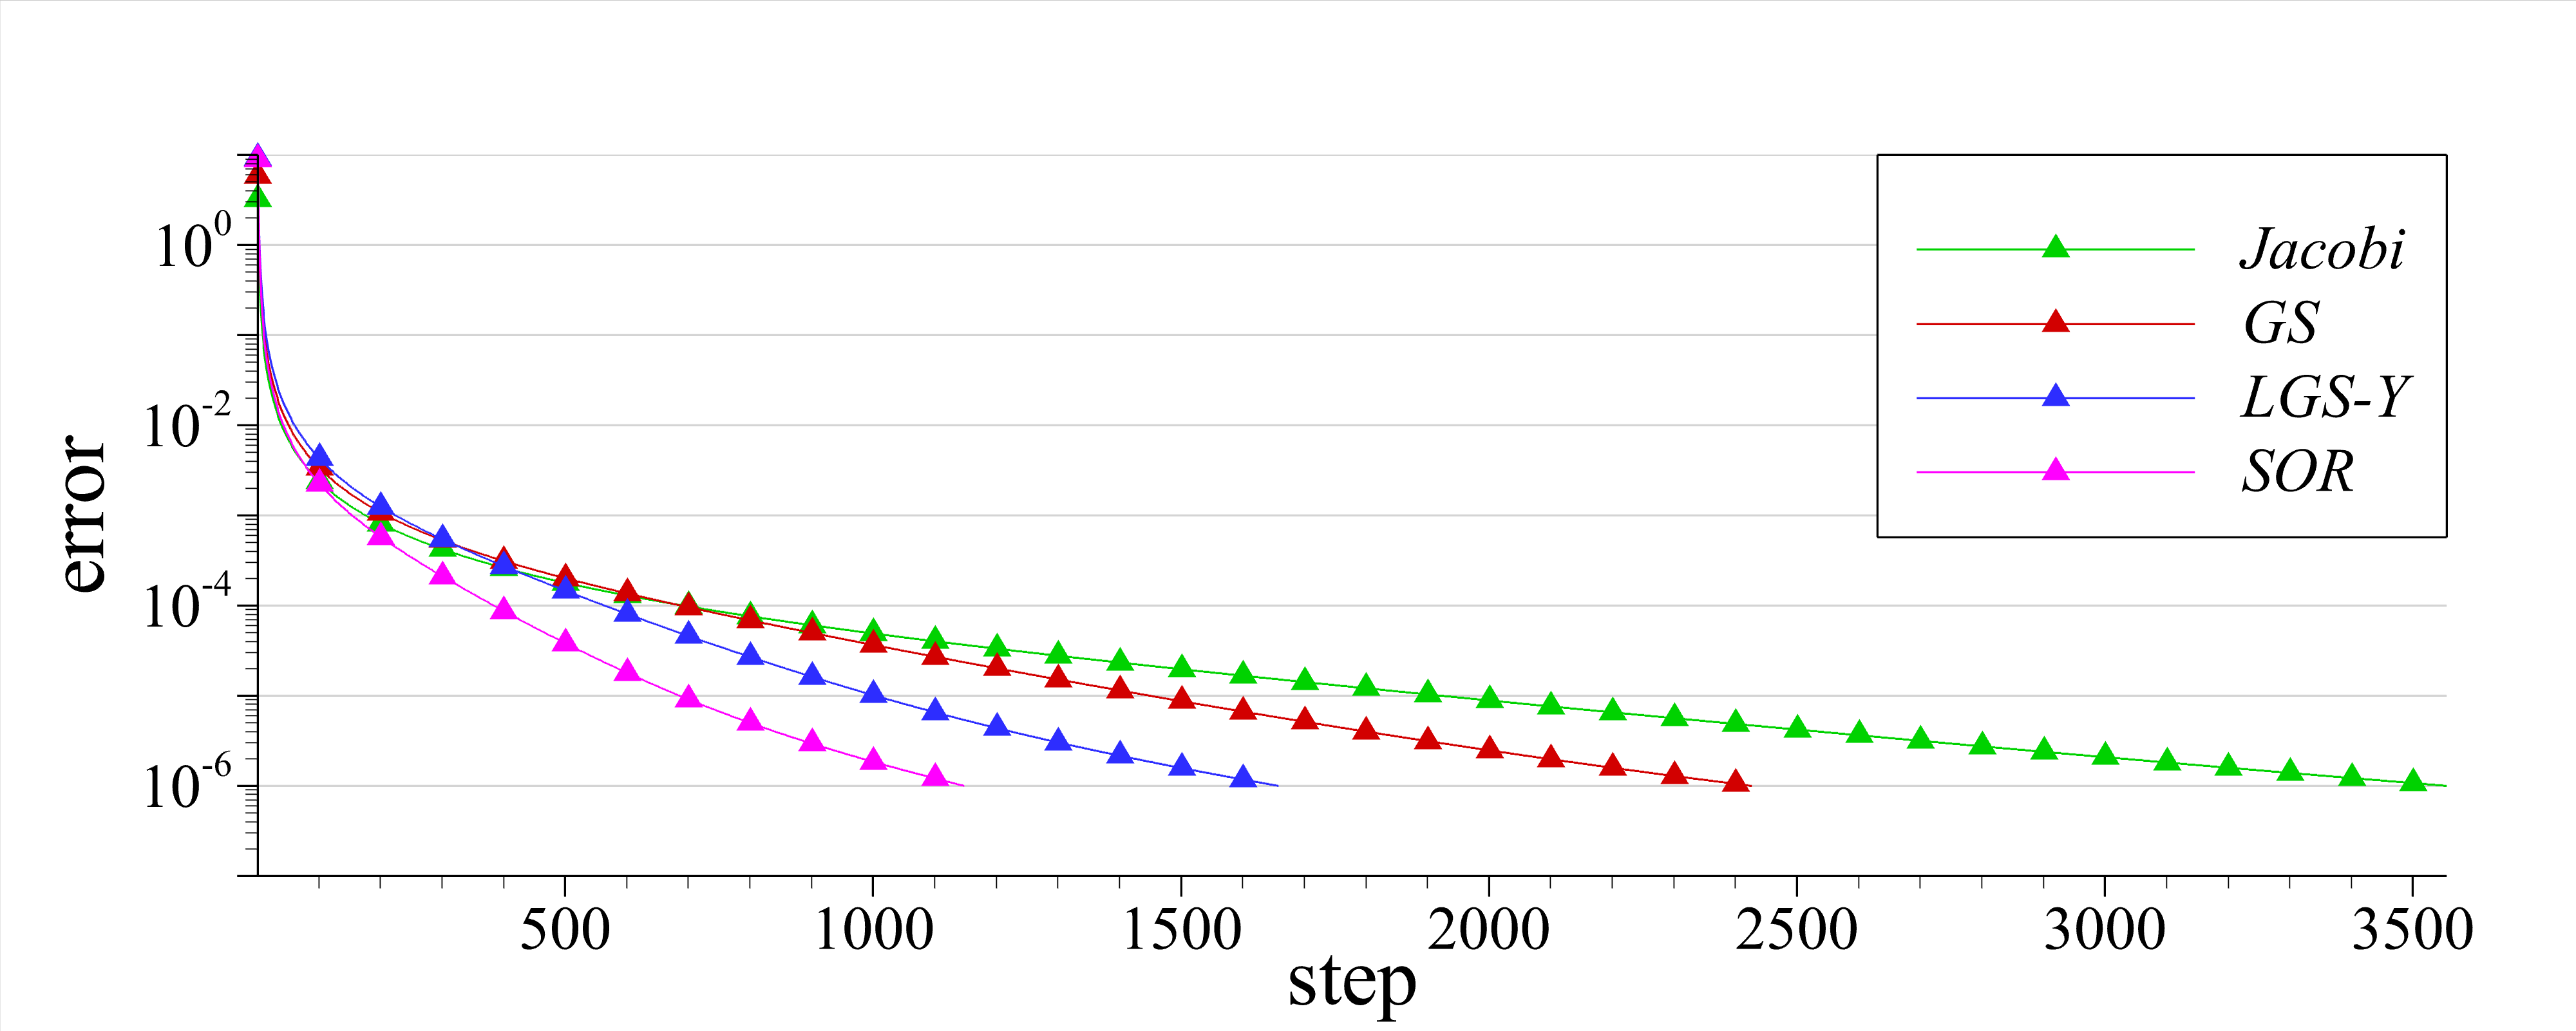
\includegraphics[width=.8\linewidth]{figure/poisson/error.png}}
	\subfigure[多重网格加速方法(含粗网格迭代)]{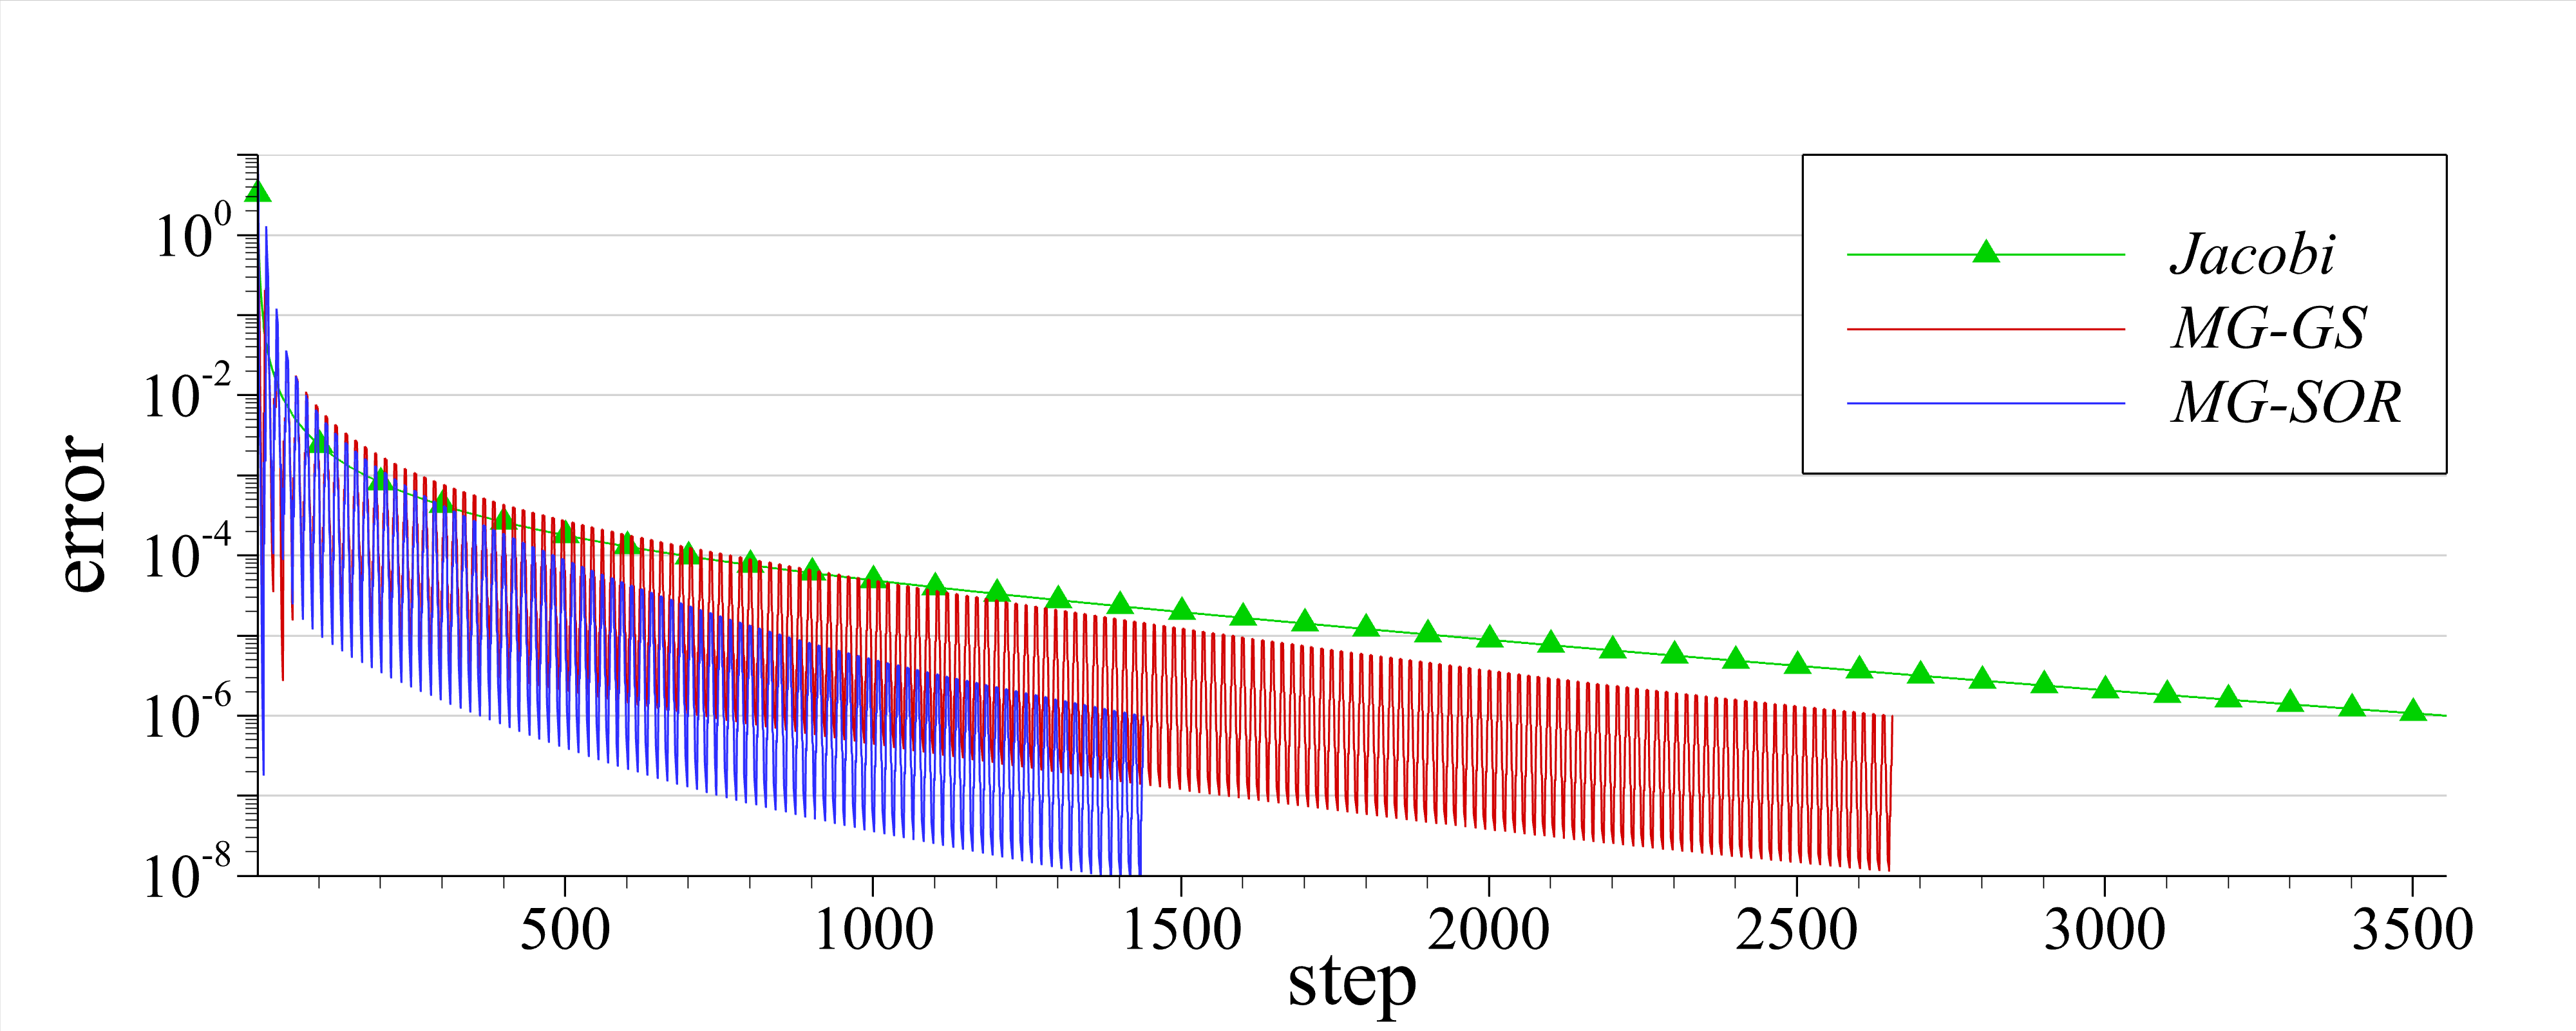
\includegraphics[width=.8\linewidth]{figure/poisson/error-MG.png}}
	\caption{\label{fig:poisson_error}误差随迭代步的收敛曲线}
\end{figure}

\begin{figure}[htbp]
	\centering
	\subfigure[Jacobi 解分布]{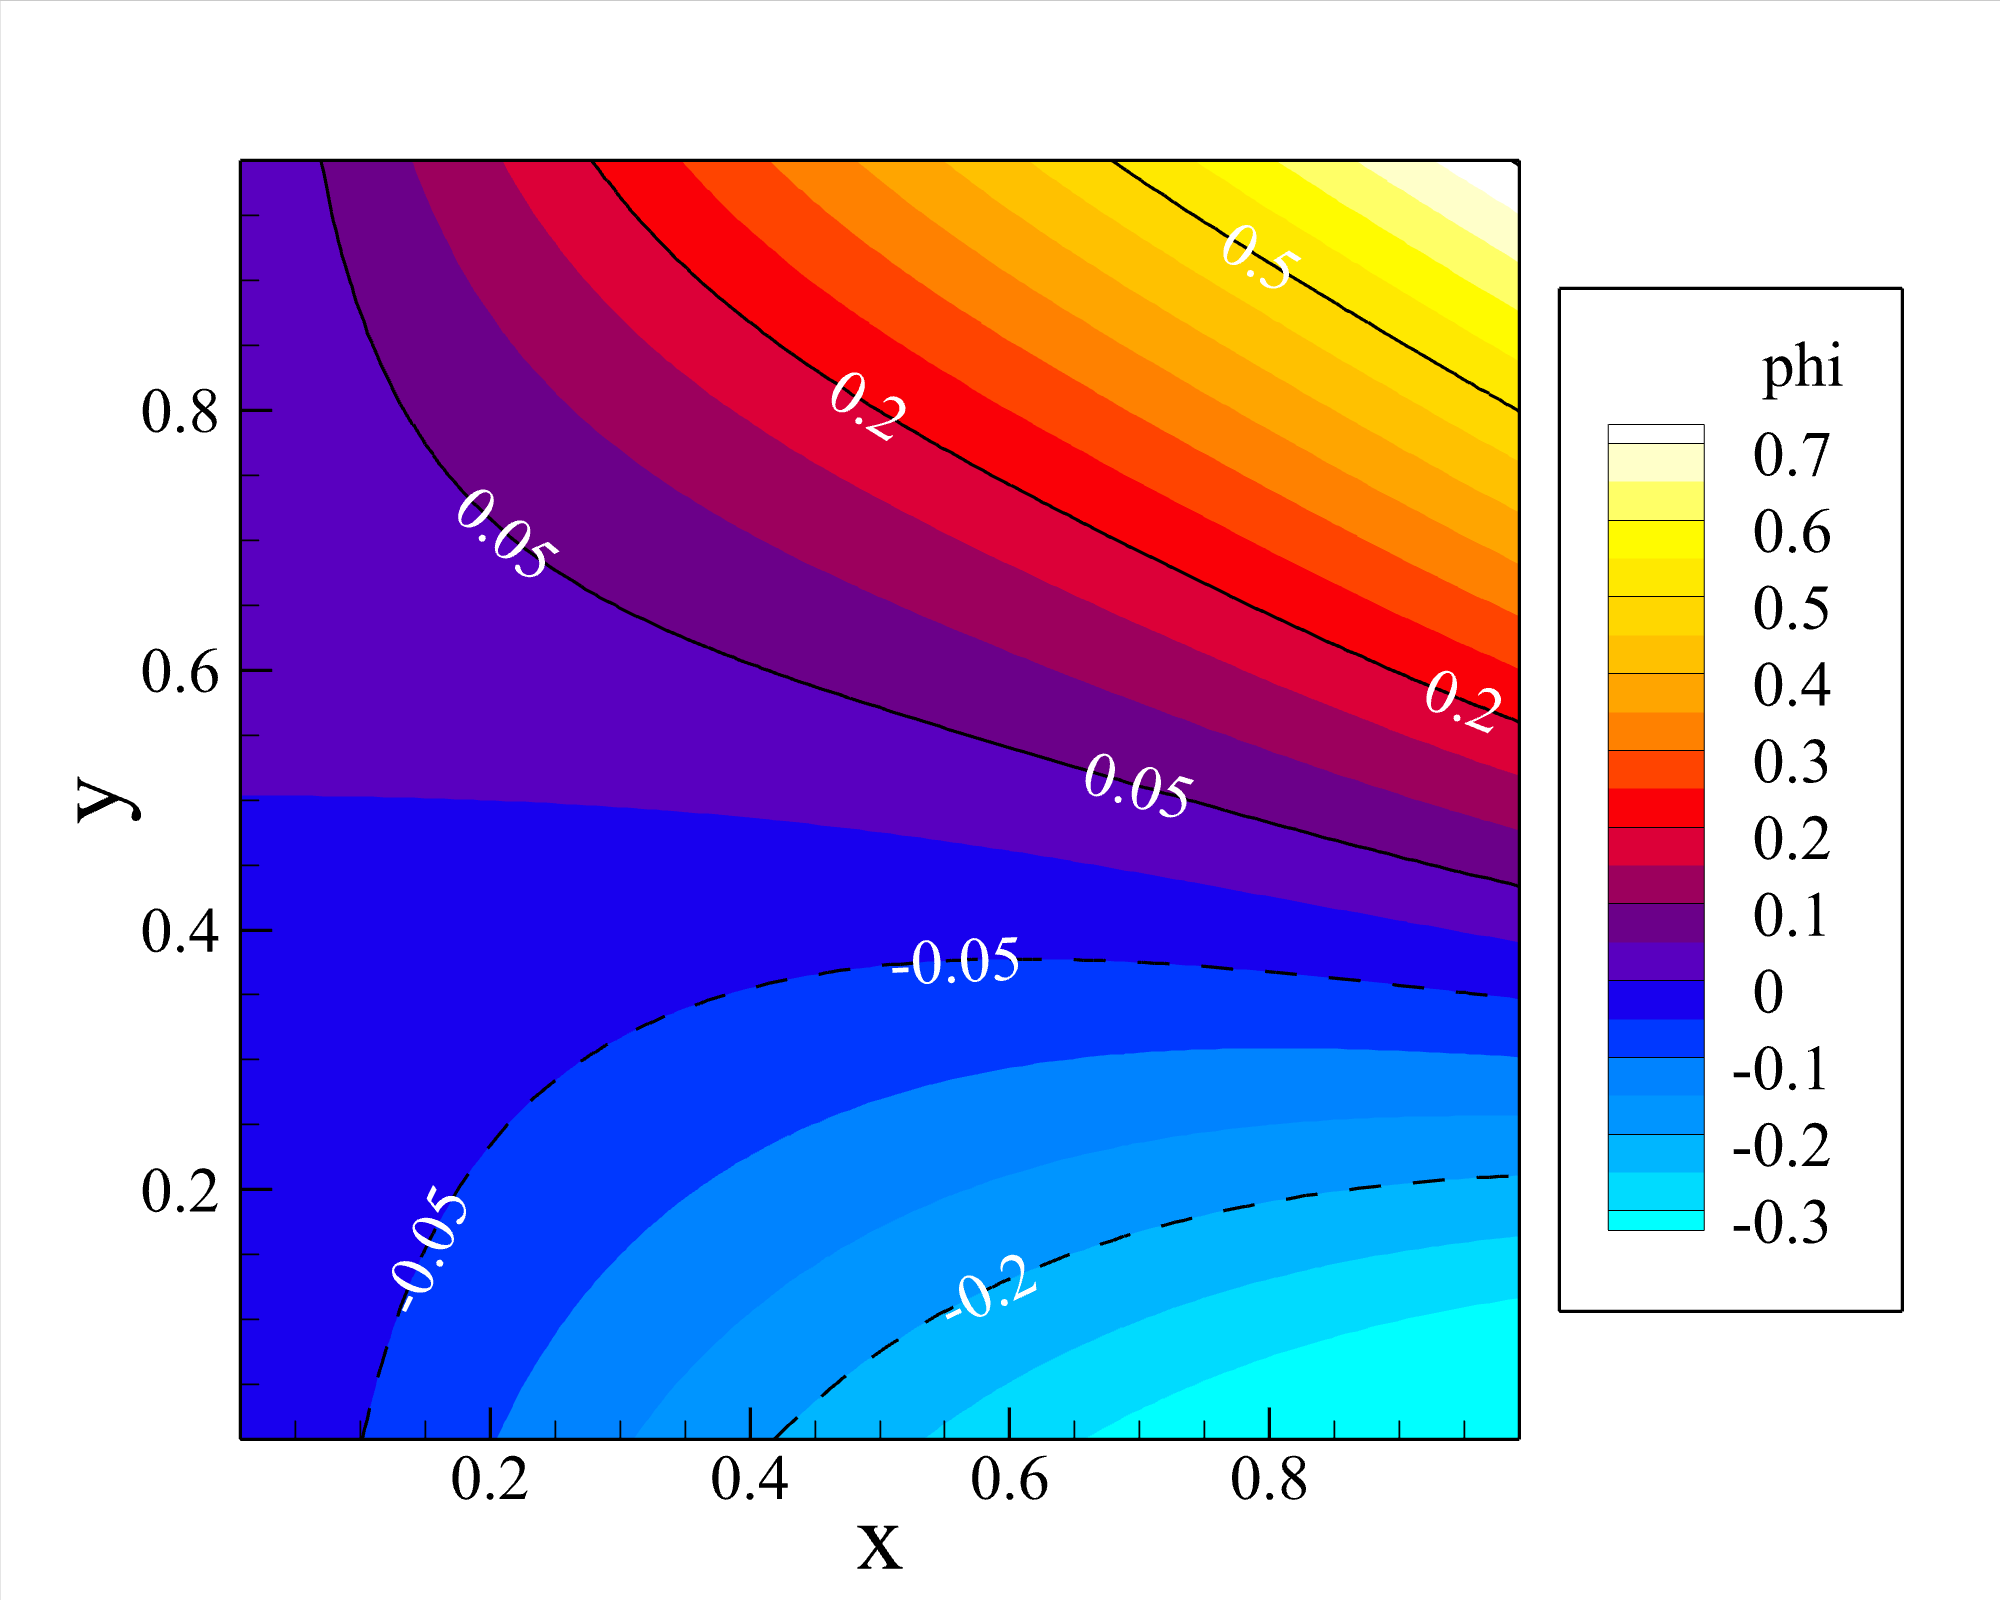
\includegraphics[width=.45\linewidth]{figure/poisson/Jacobi-sol.png}}
	\subfigure[Jacobi 残差分布]{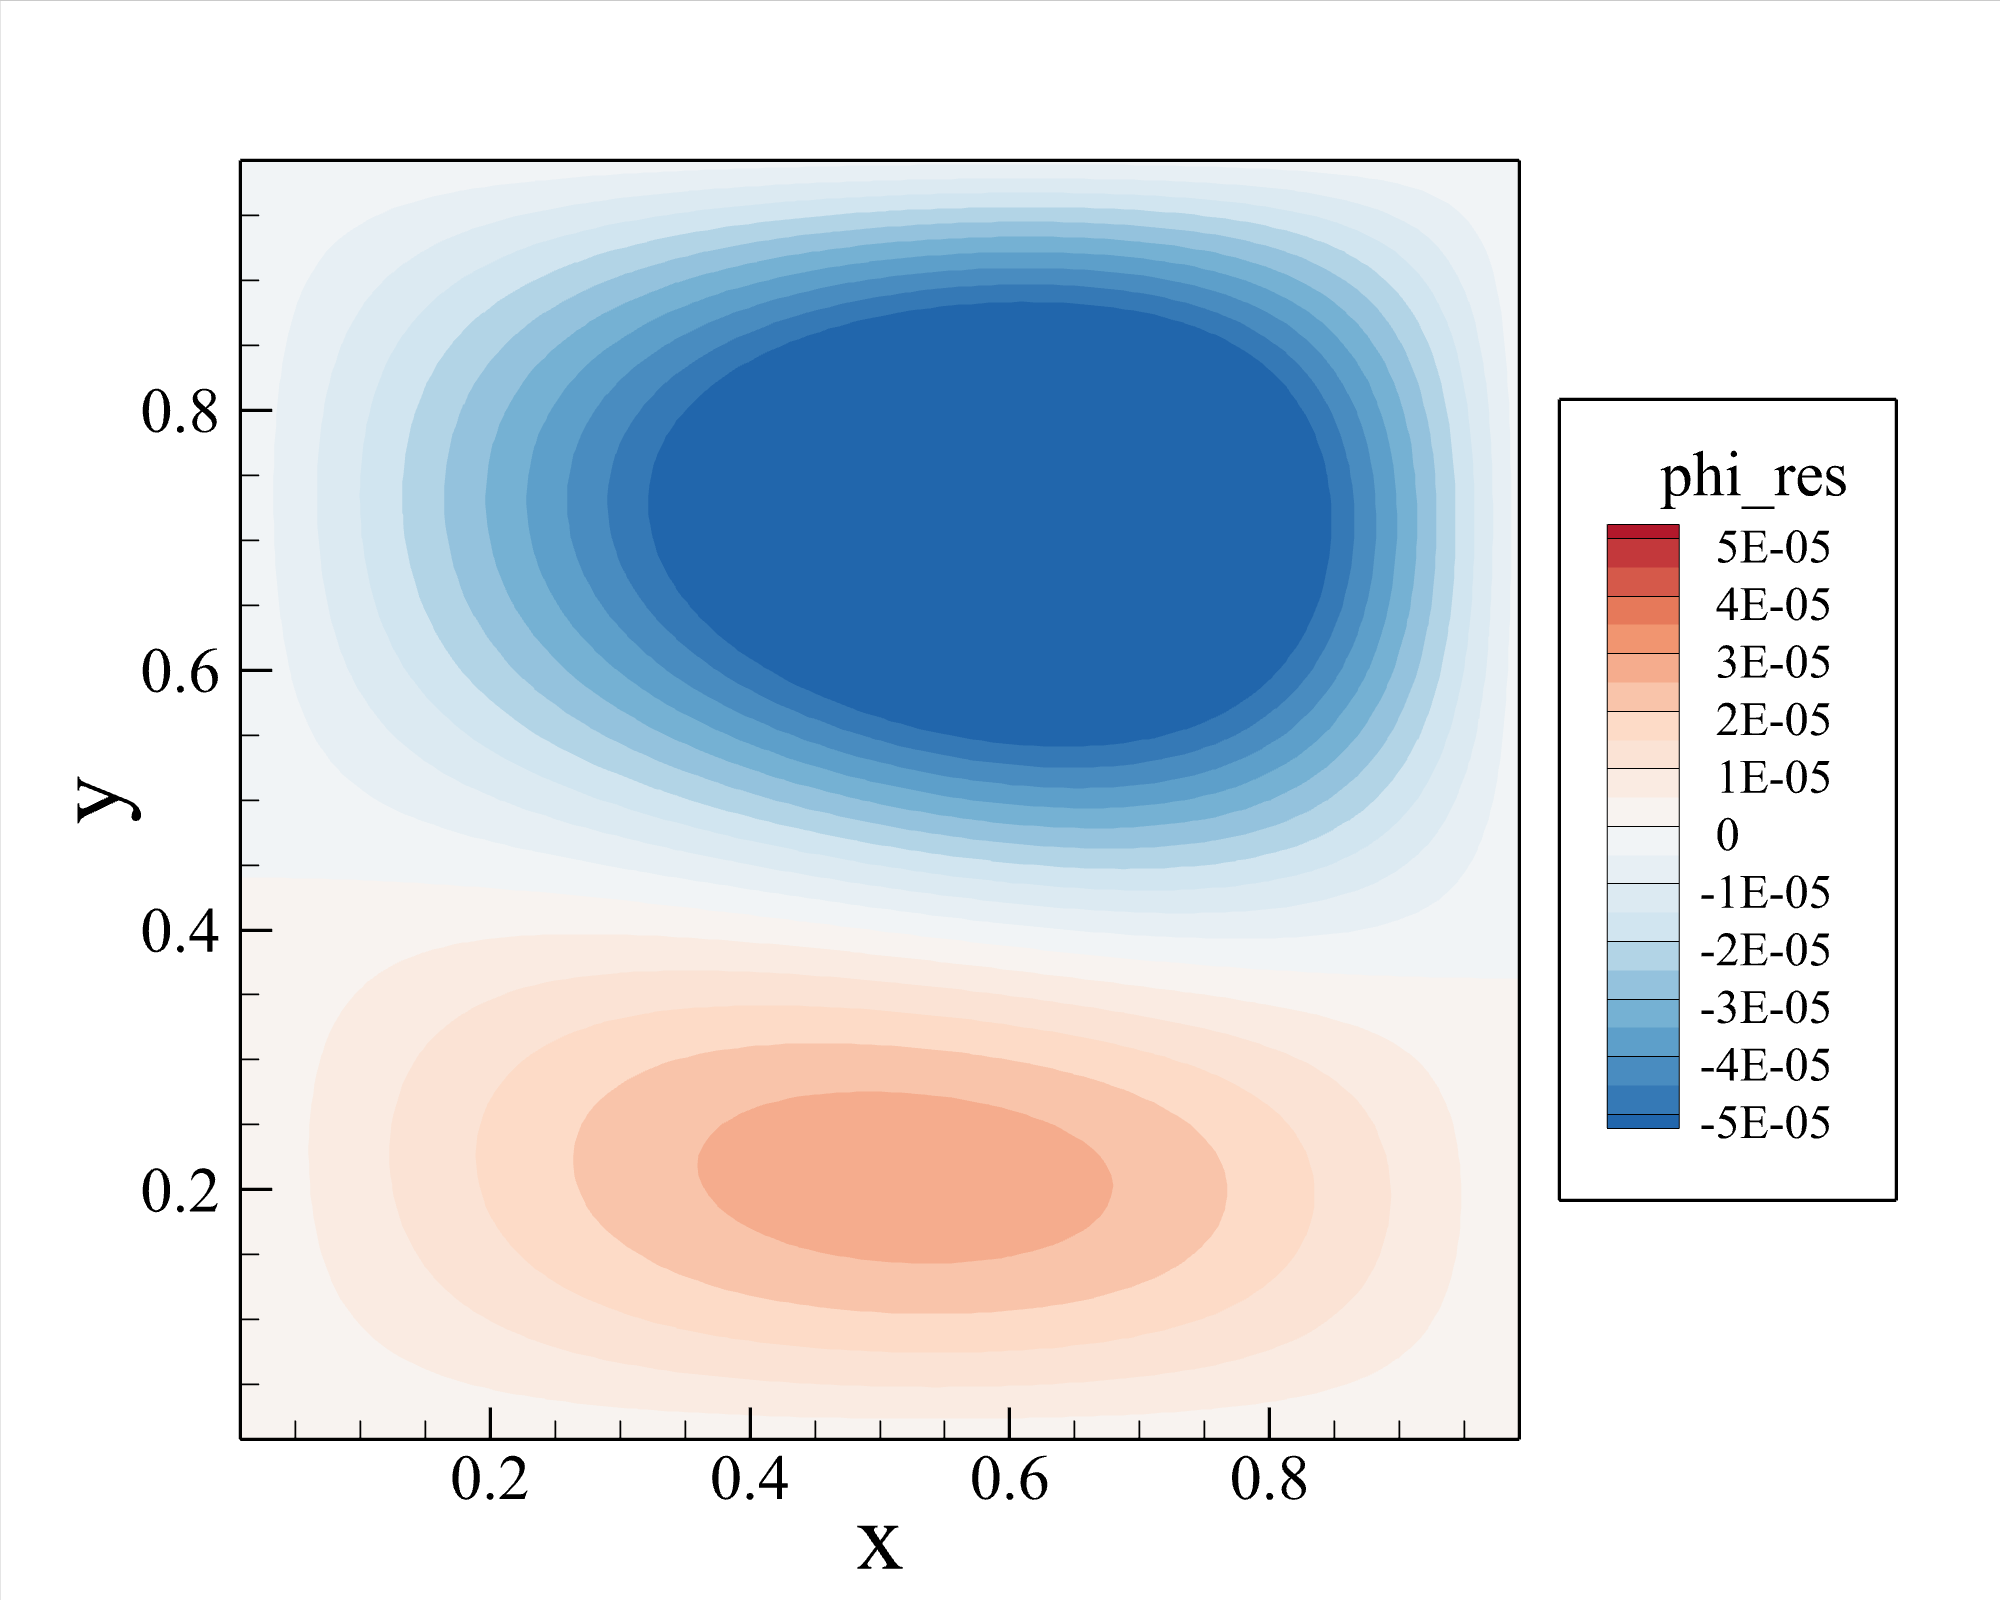
\includegraphics[width=.45\linewidth]{figure/poisson/Jacobi-res.png}}

	\subfigure[GS 解分布]{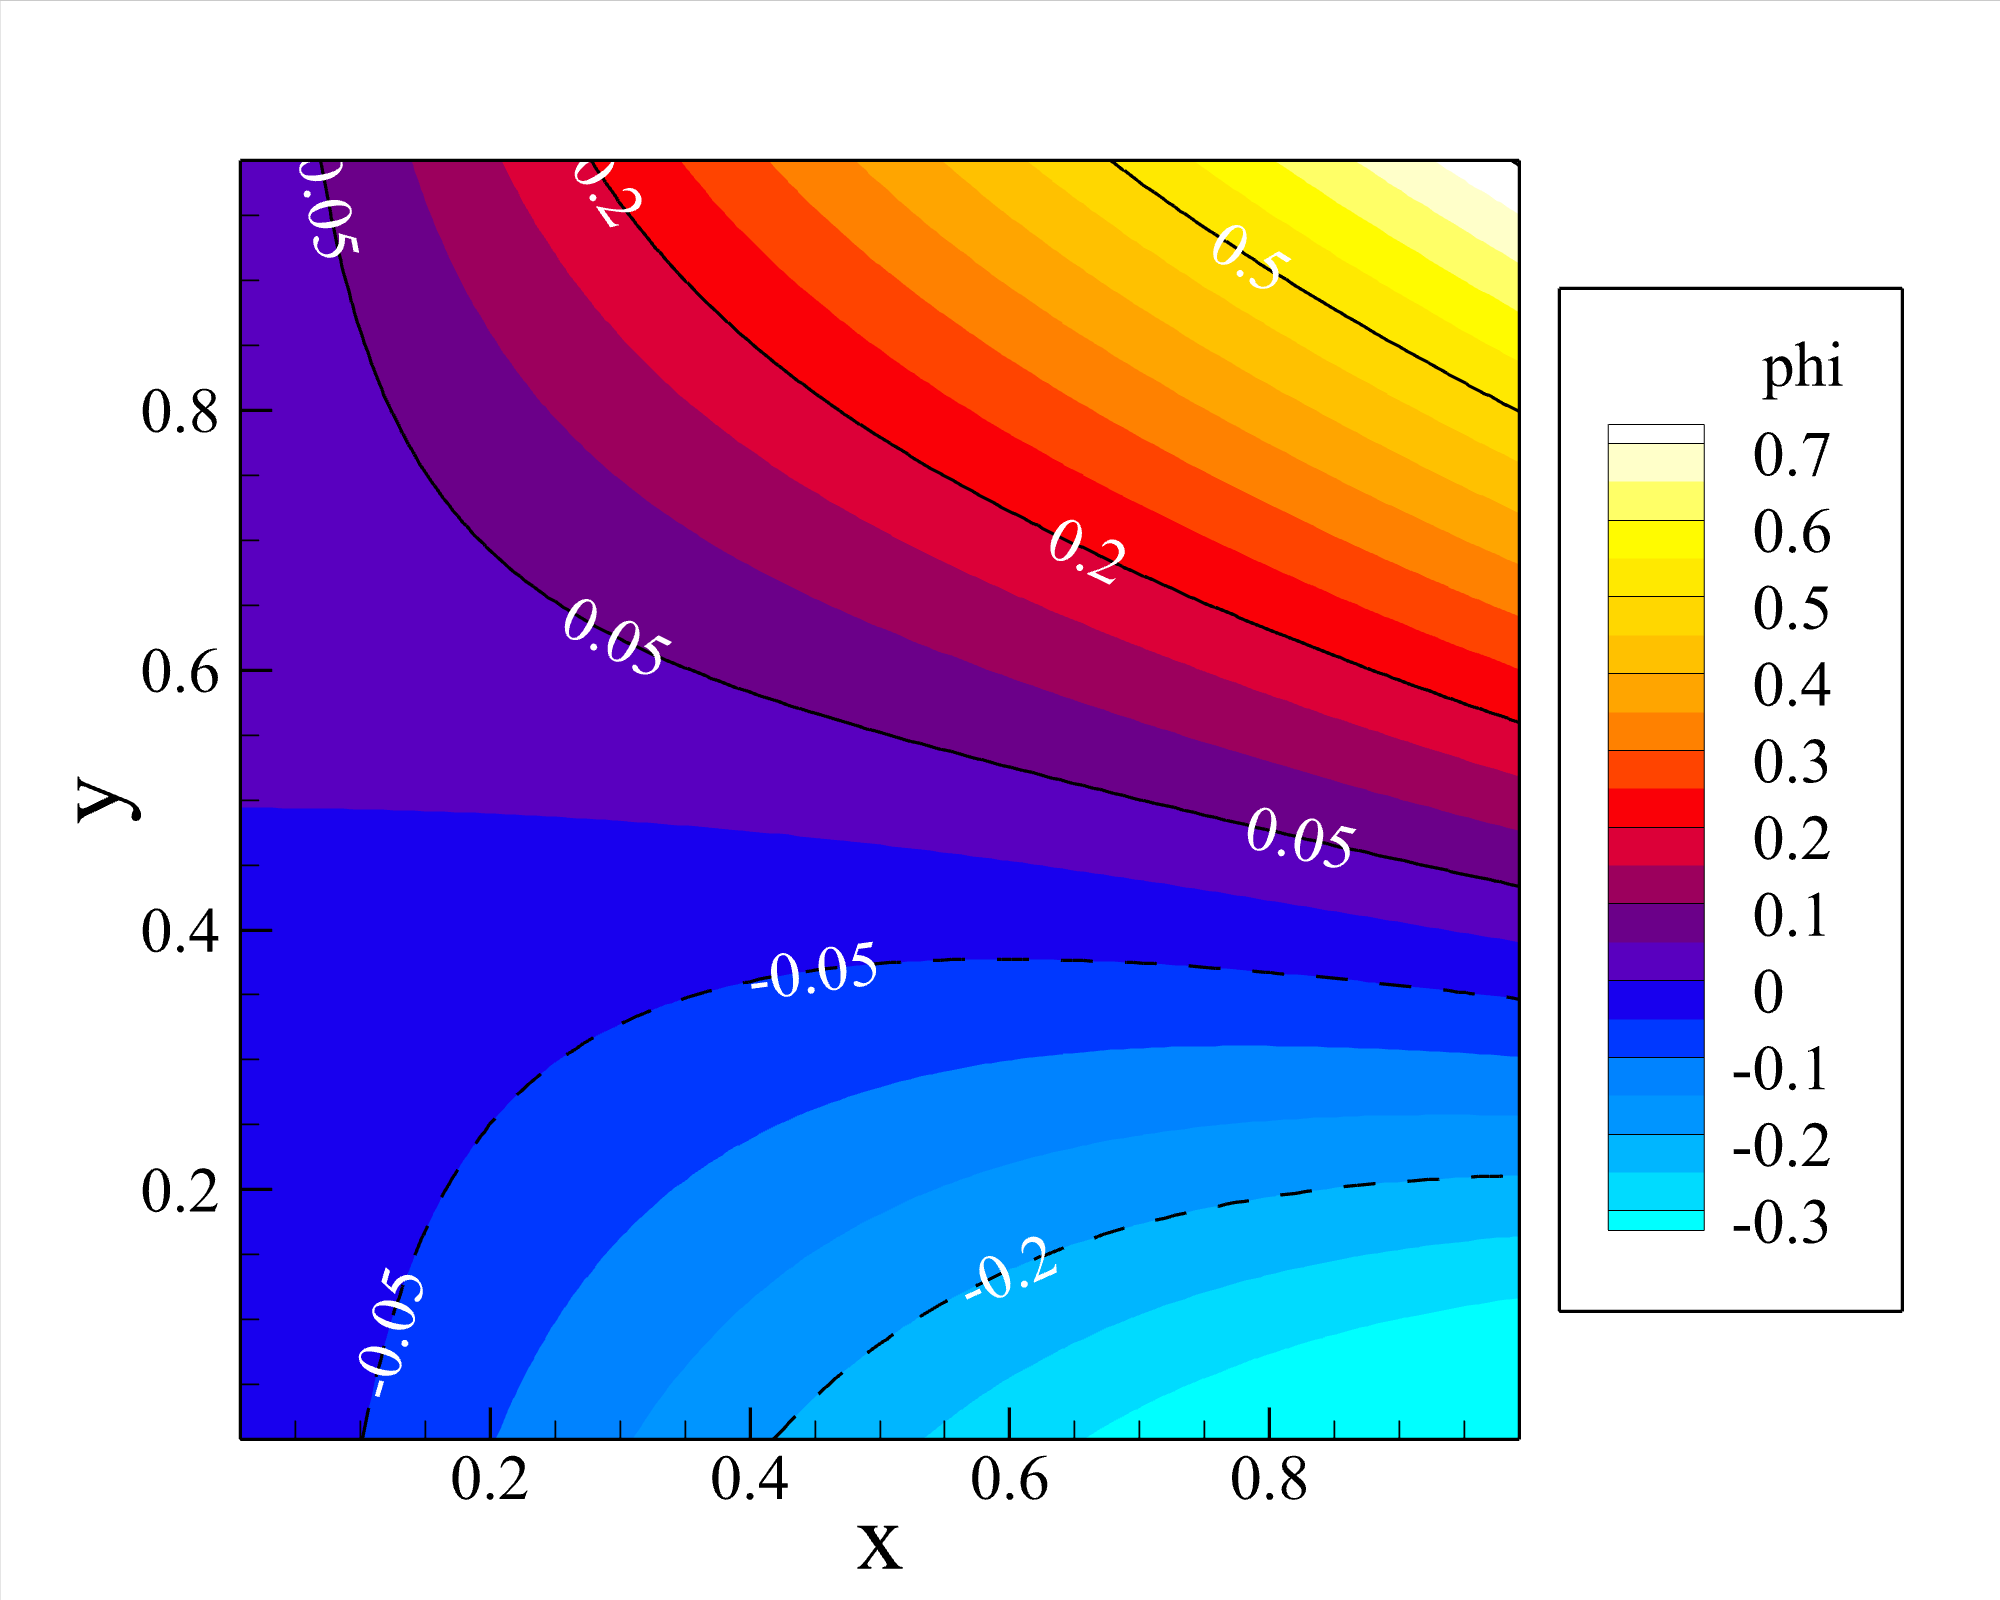
\includegraphics[width=.45\linewidth]{figure/poisson/GS-sol.png}}
	\subfigure[GS 残差分布]{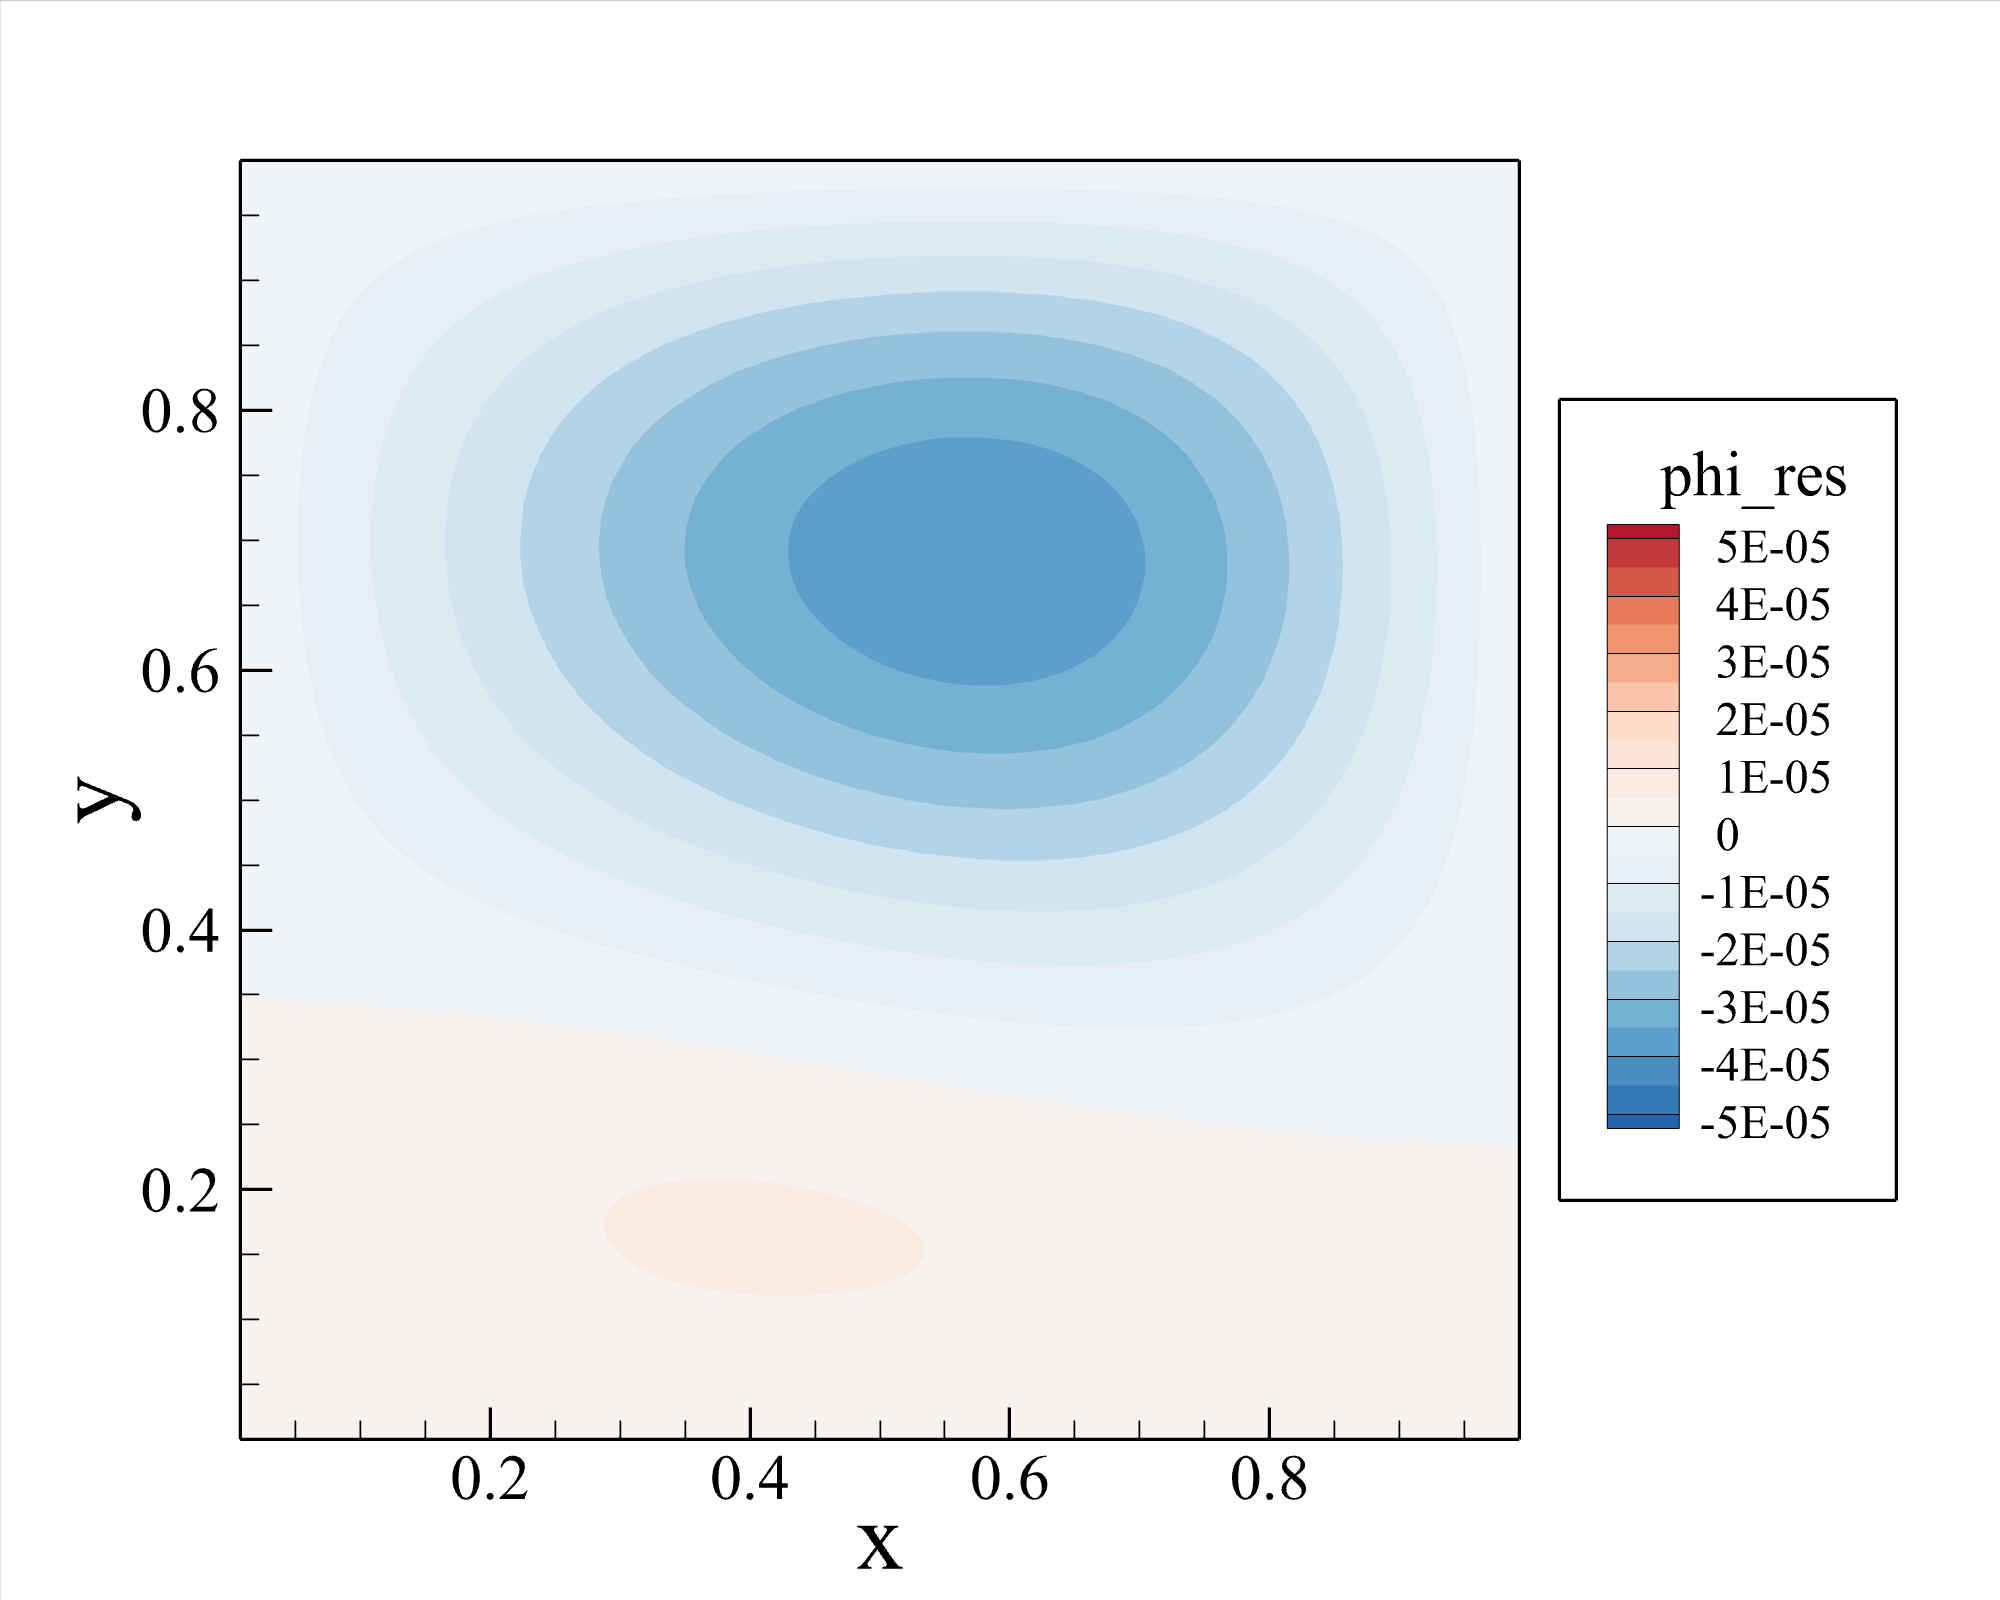
\includegraphics[width=.45\linewidth]{figure/poisson/GS-res.png}}

	\subfigure[LGS-Y 解分布]{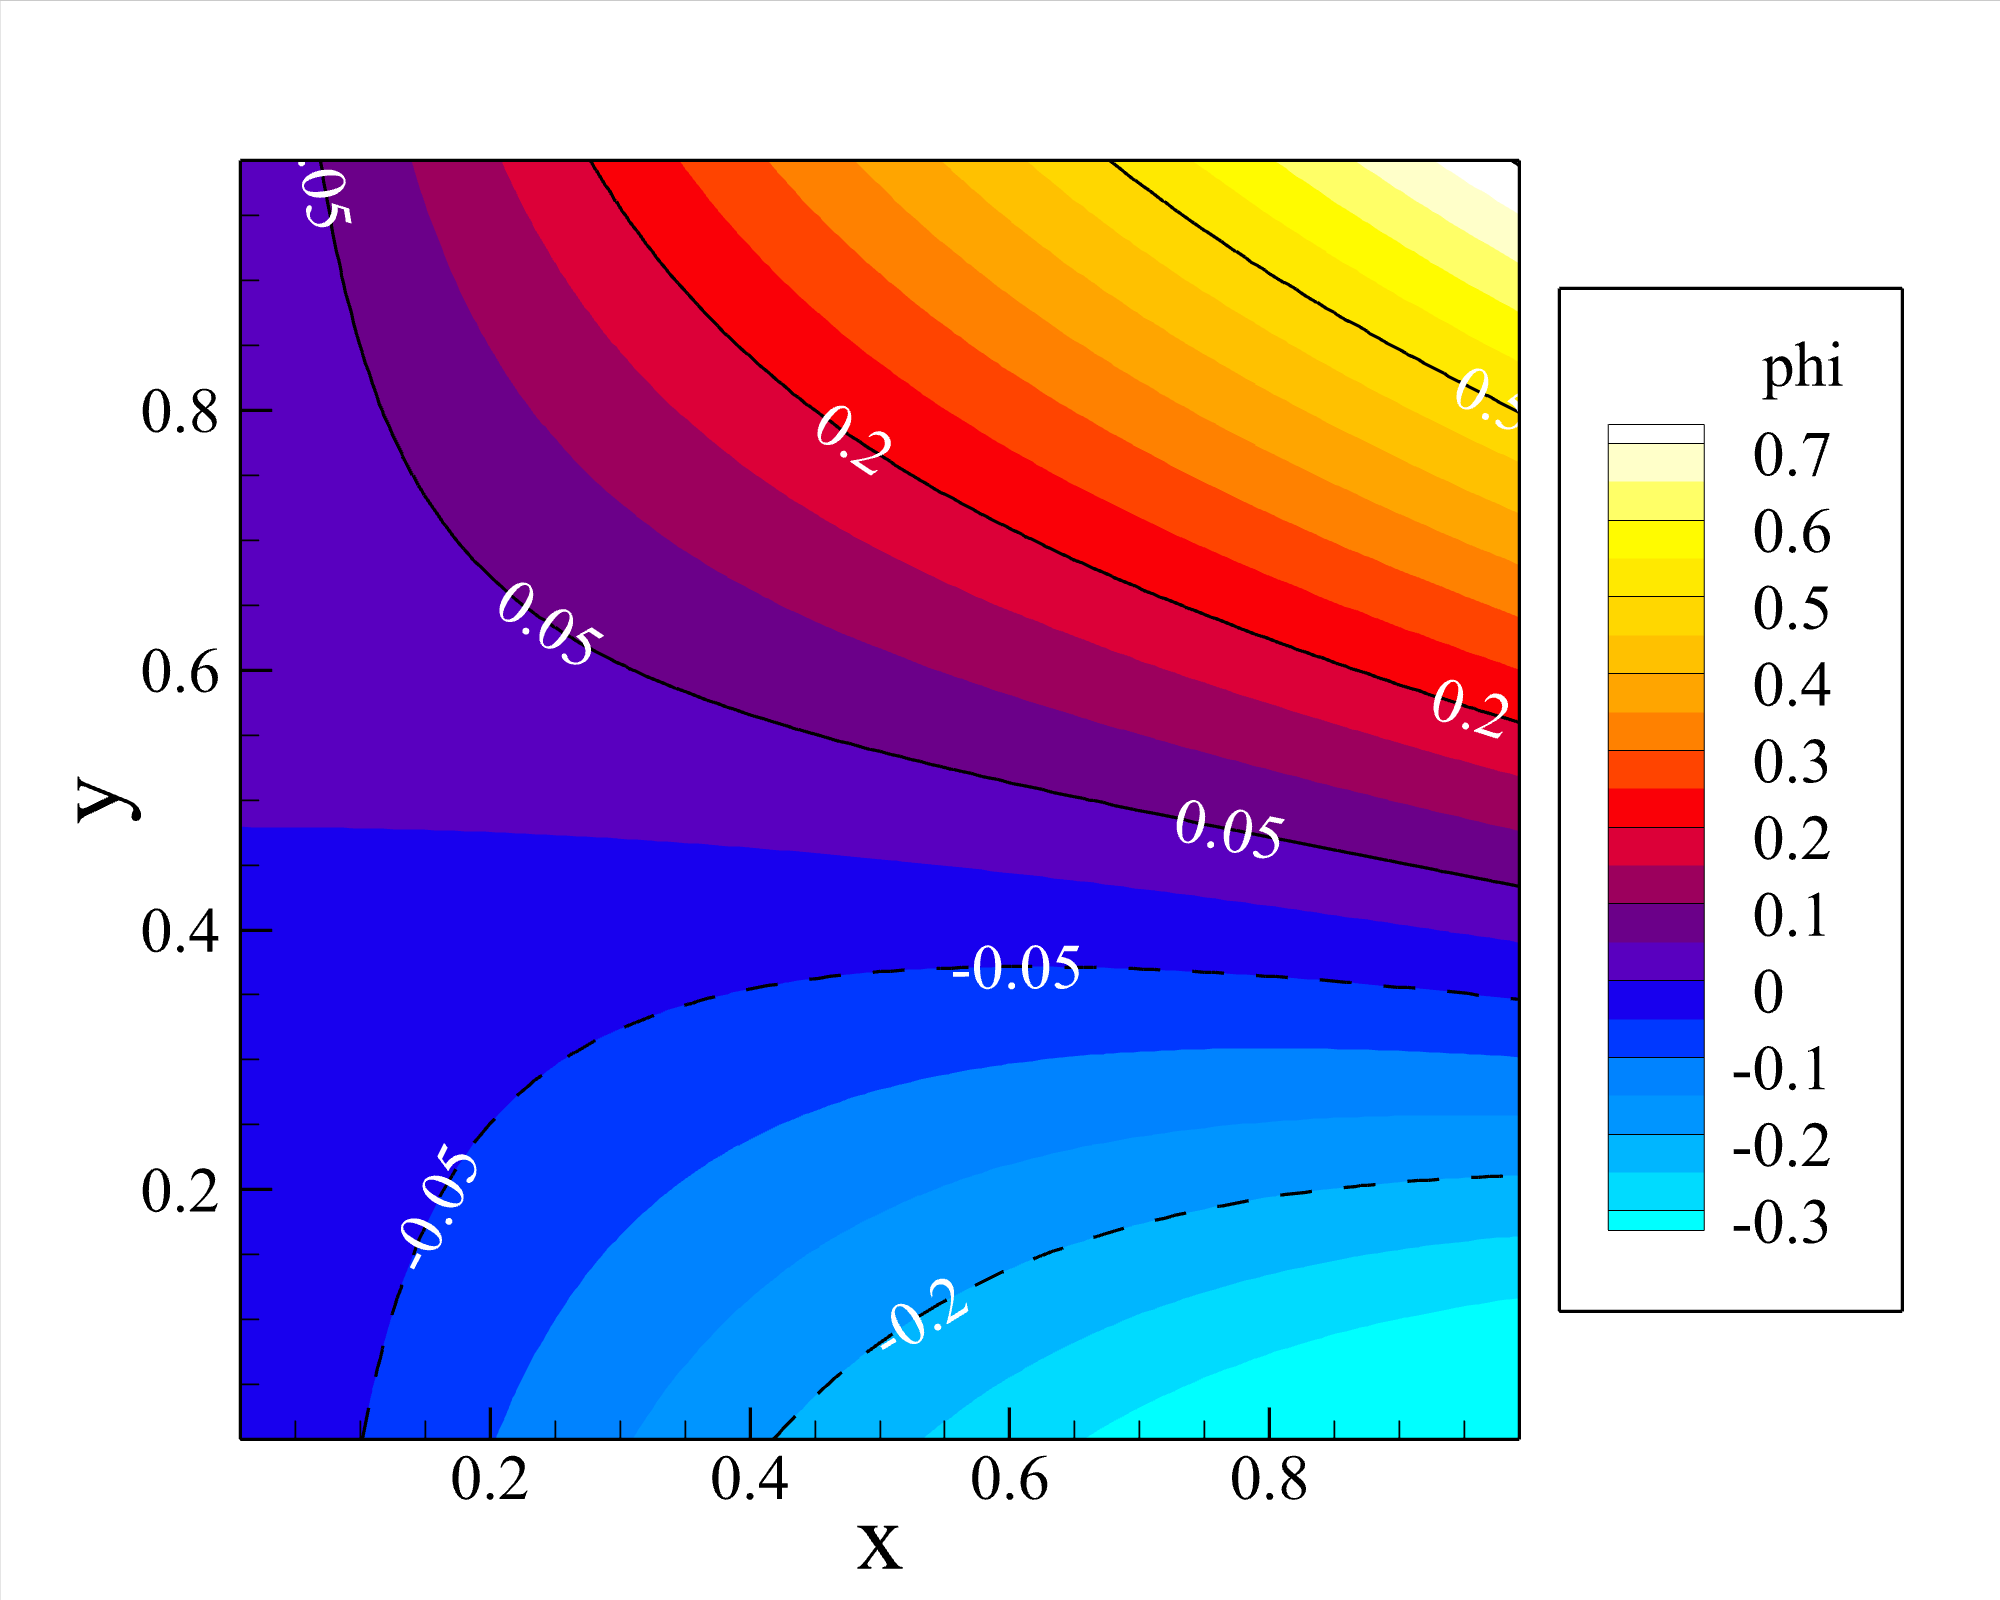
\includegraphics[width=.45\linewidth]{figure/poisson/LGSY-sol.png}}
	\subfigure[LGS-Y 残差分布]{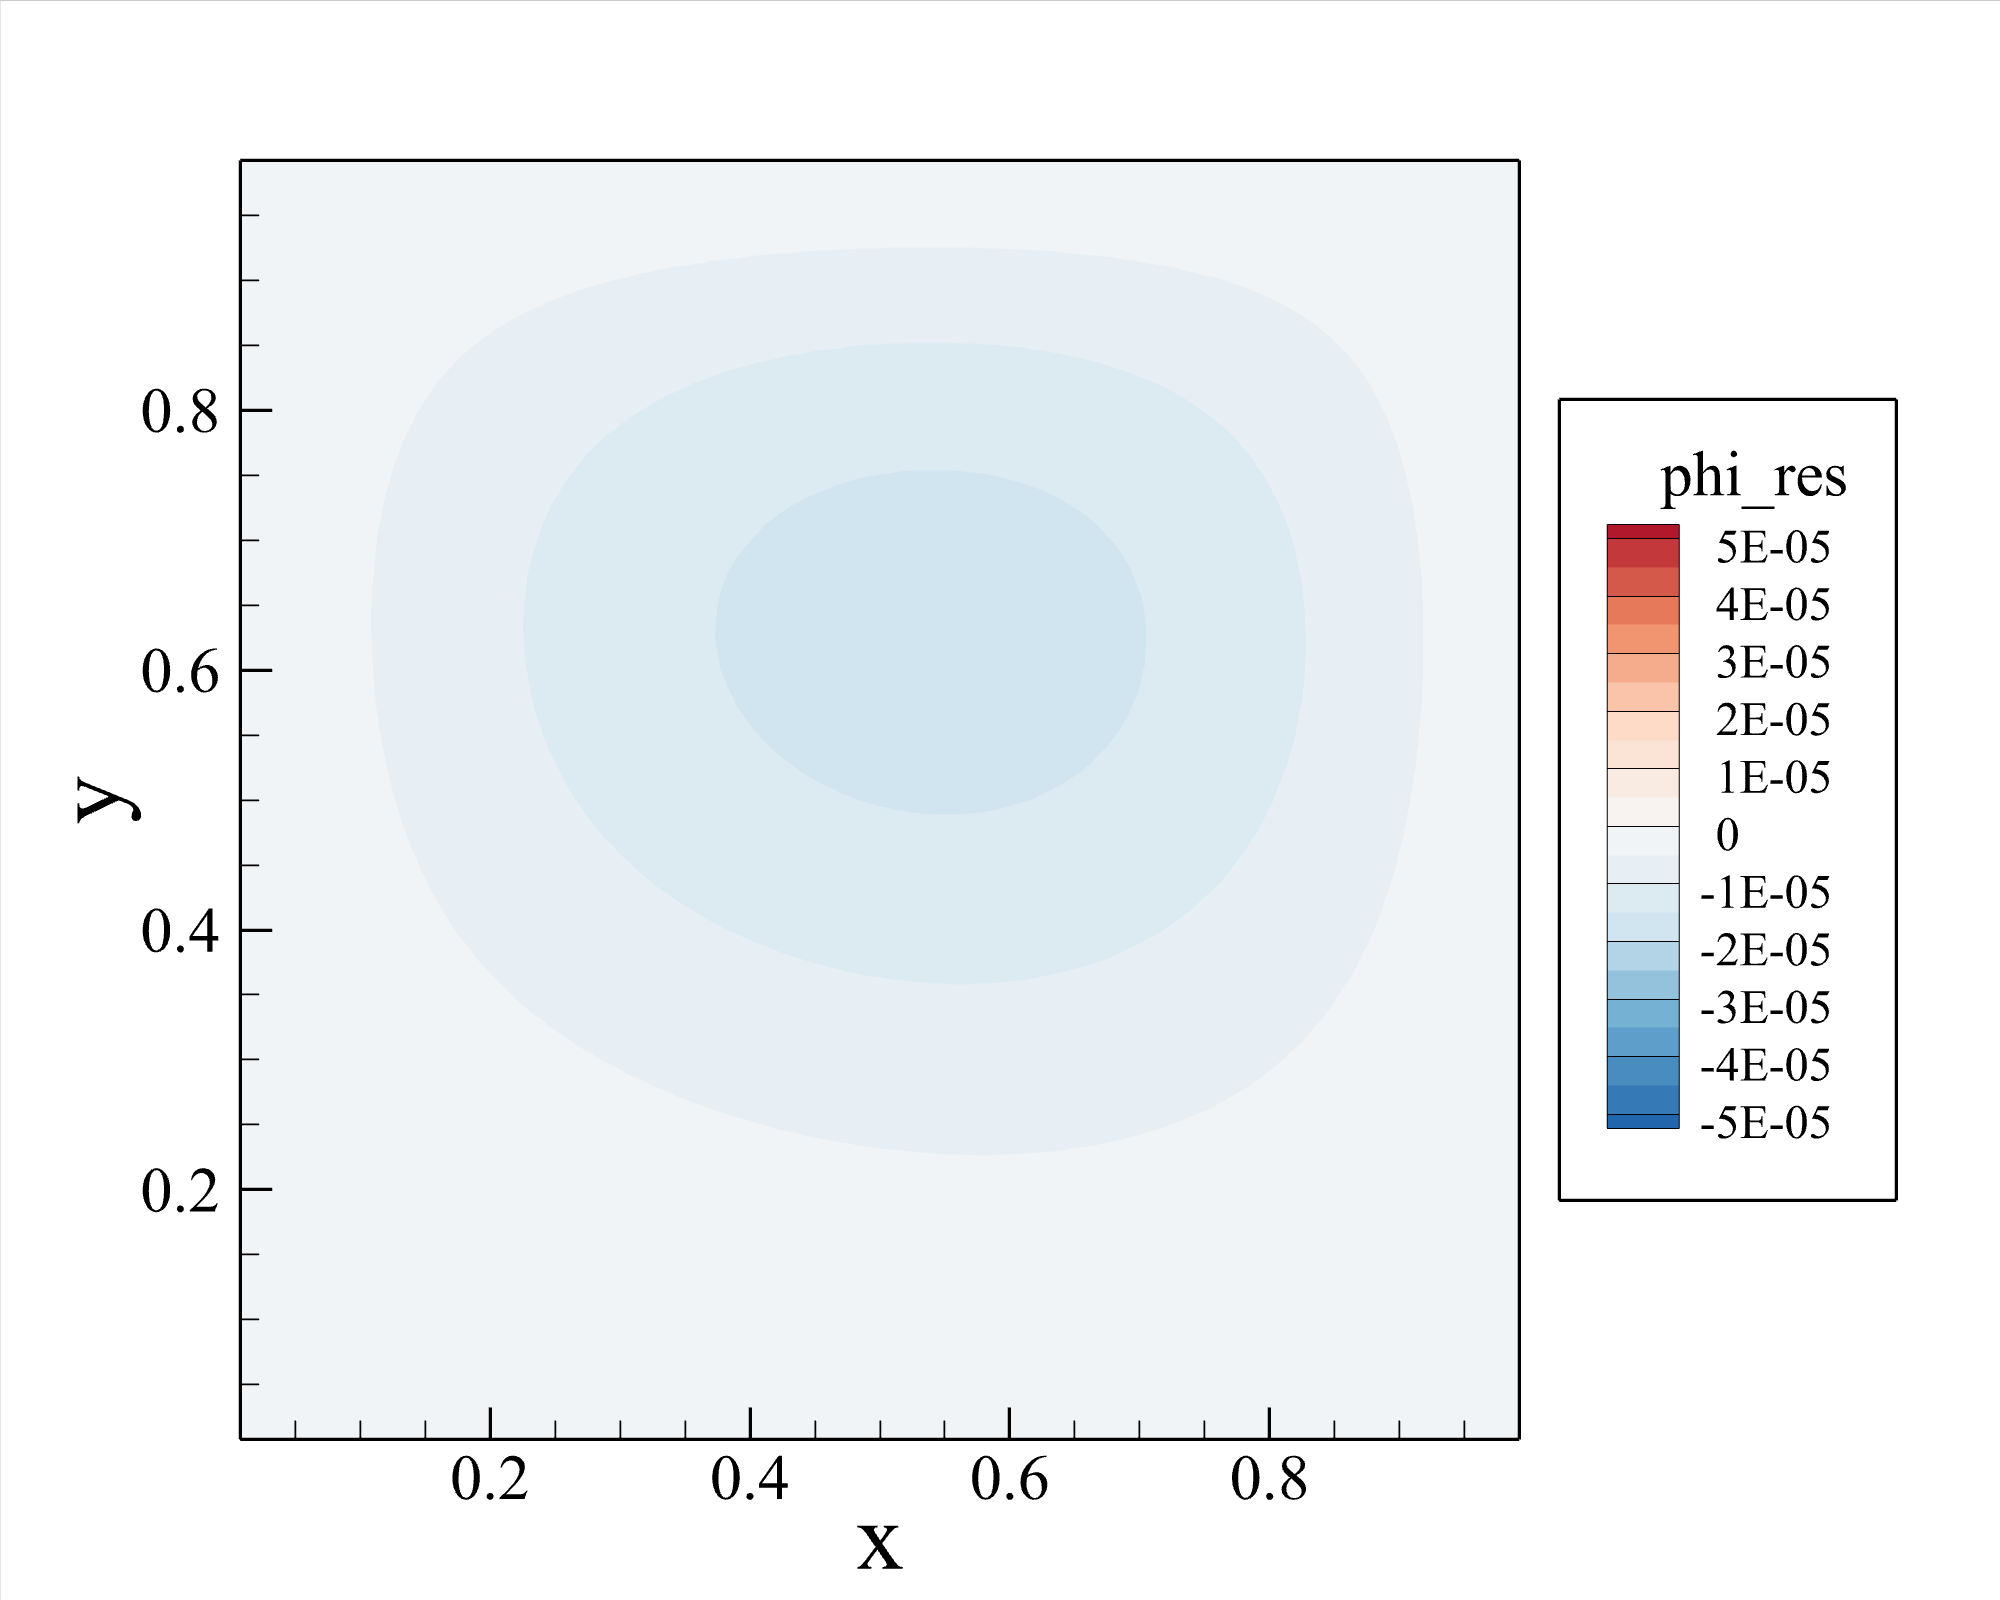
\includegraphics[width=.45\linewidth]{figure/poisson/LGSY-res.png}}

	\caption{\label{fig:poisson1}各种迭代法求解Poisson方程的结果与残差}
\end{figure}

\begin{figure}[htbp]
	\centering

	\subfigure[SOR 解分布]{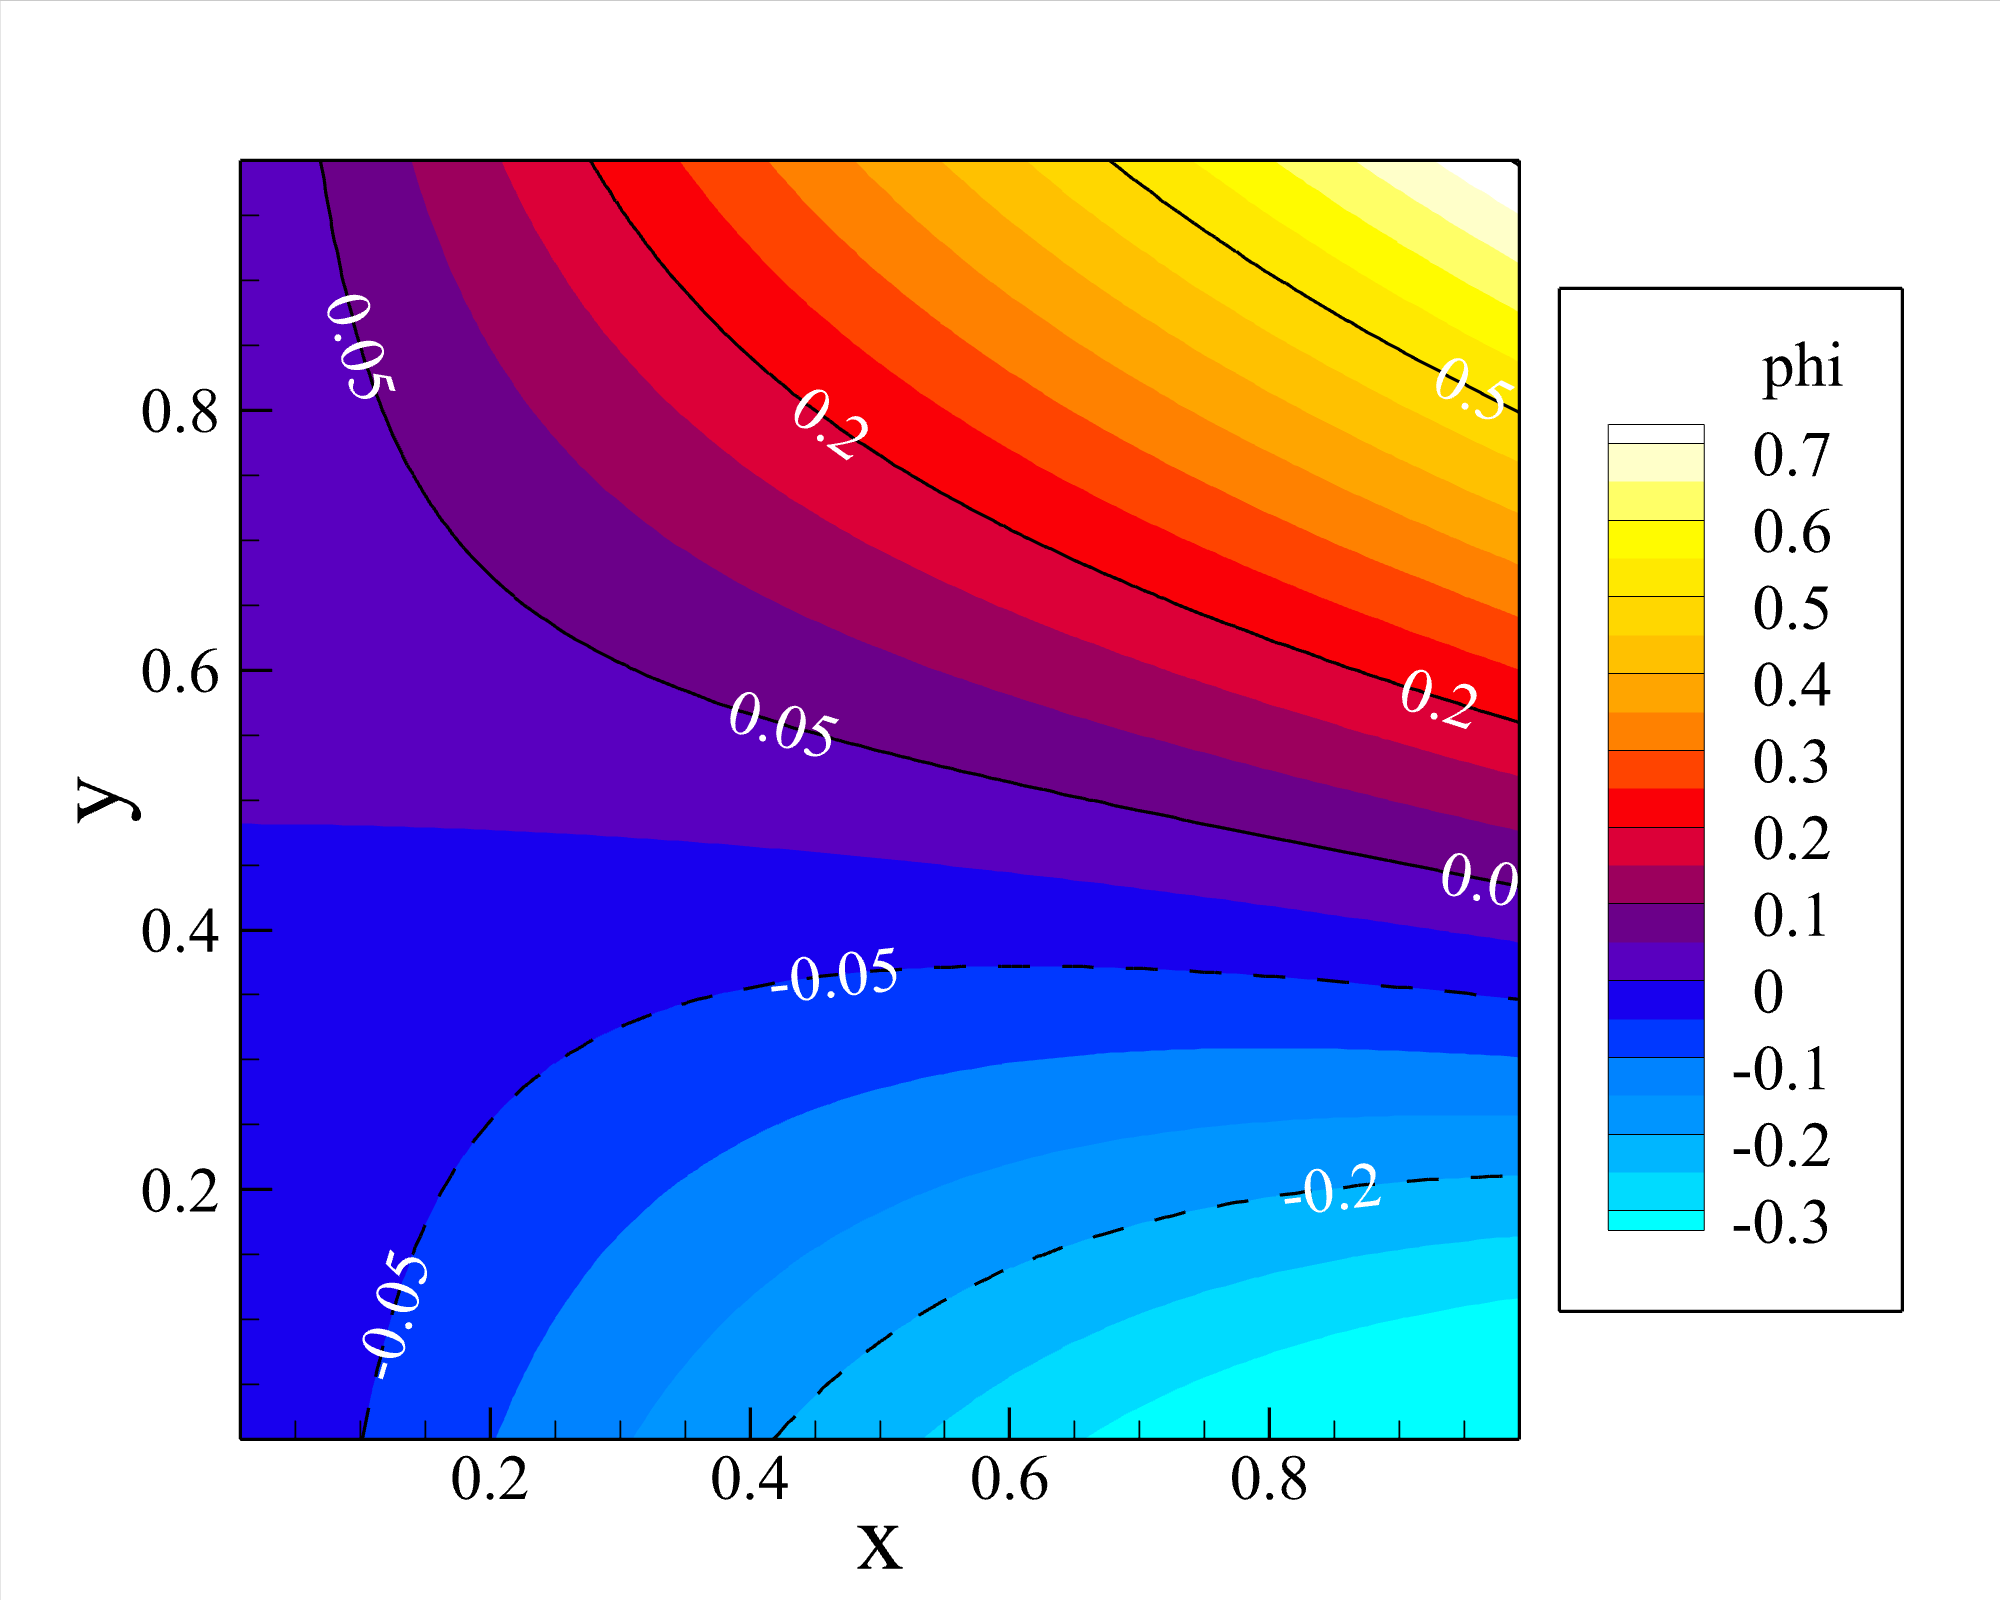
\includegraphics[width=.45\linewidth]{figure/poisson/SOR-sol.png}}
	\subfigure[SOR 残差分布]{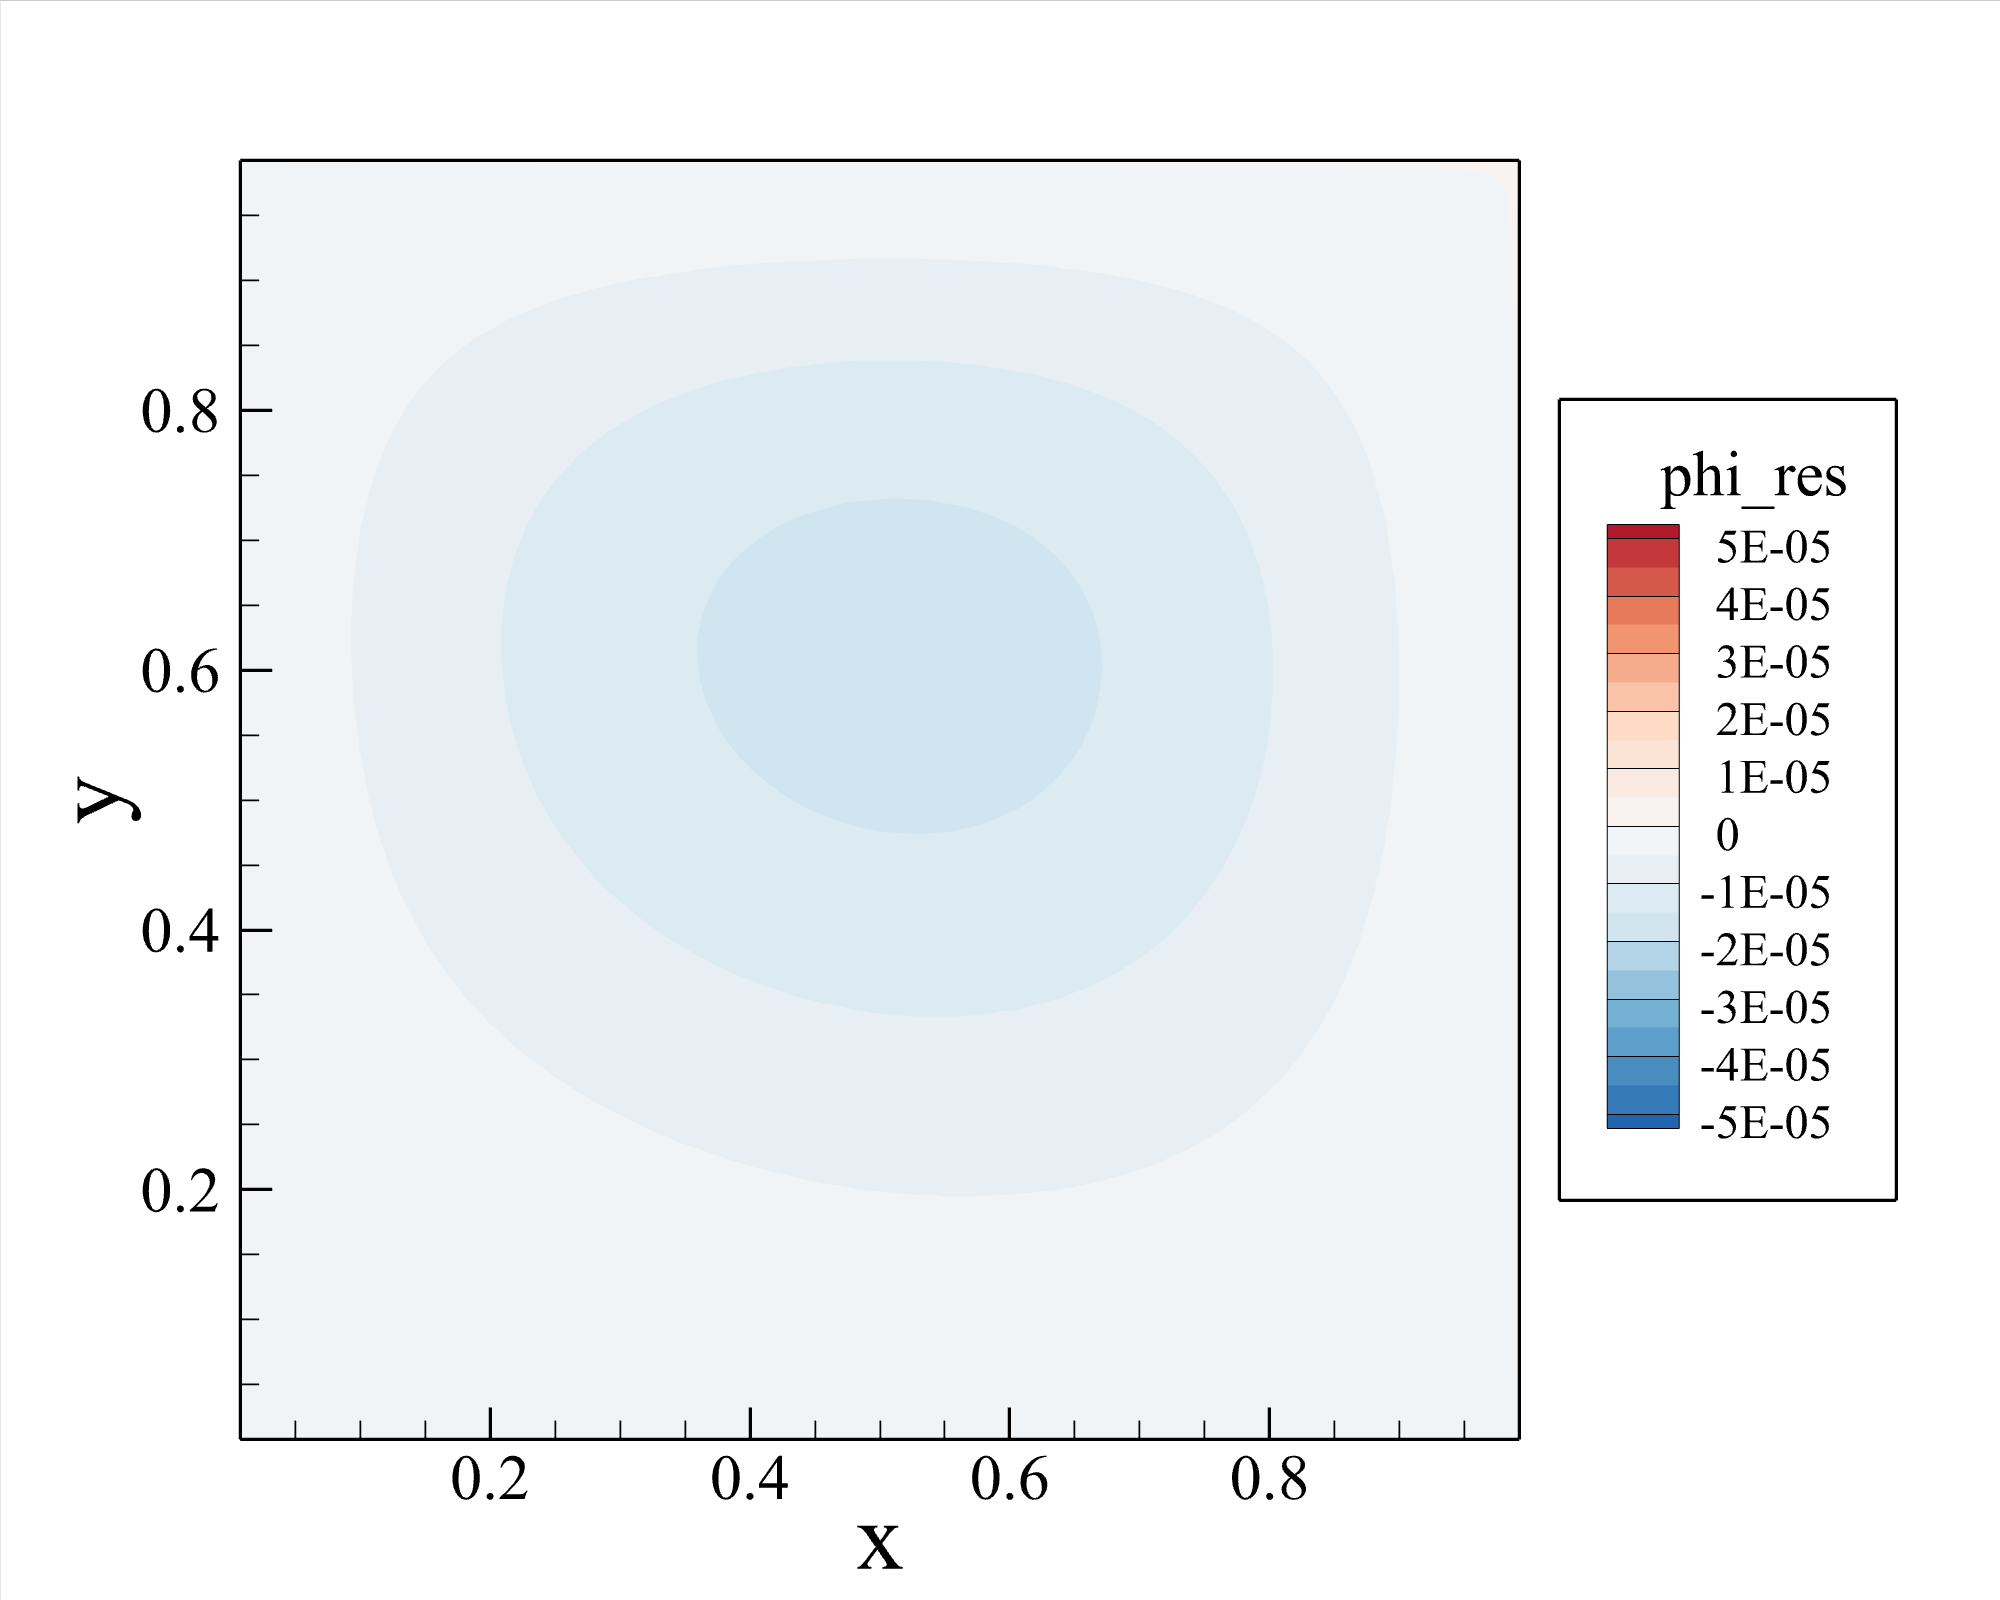
\includegraphics[width=.45\linewidth]{figure/poisson/SOR-res.png}}

	\subfigure[MG-GS 解分布]{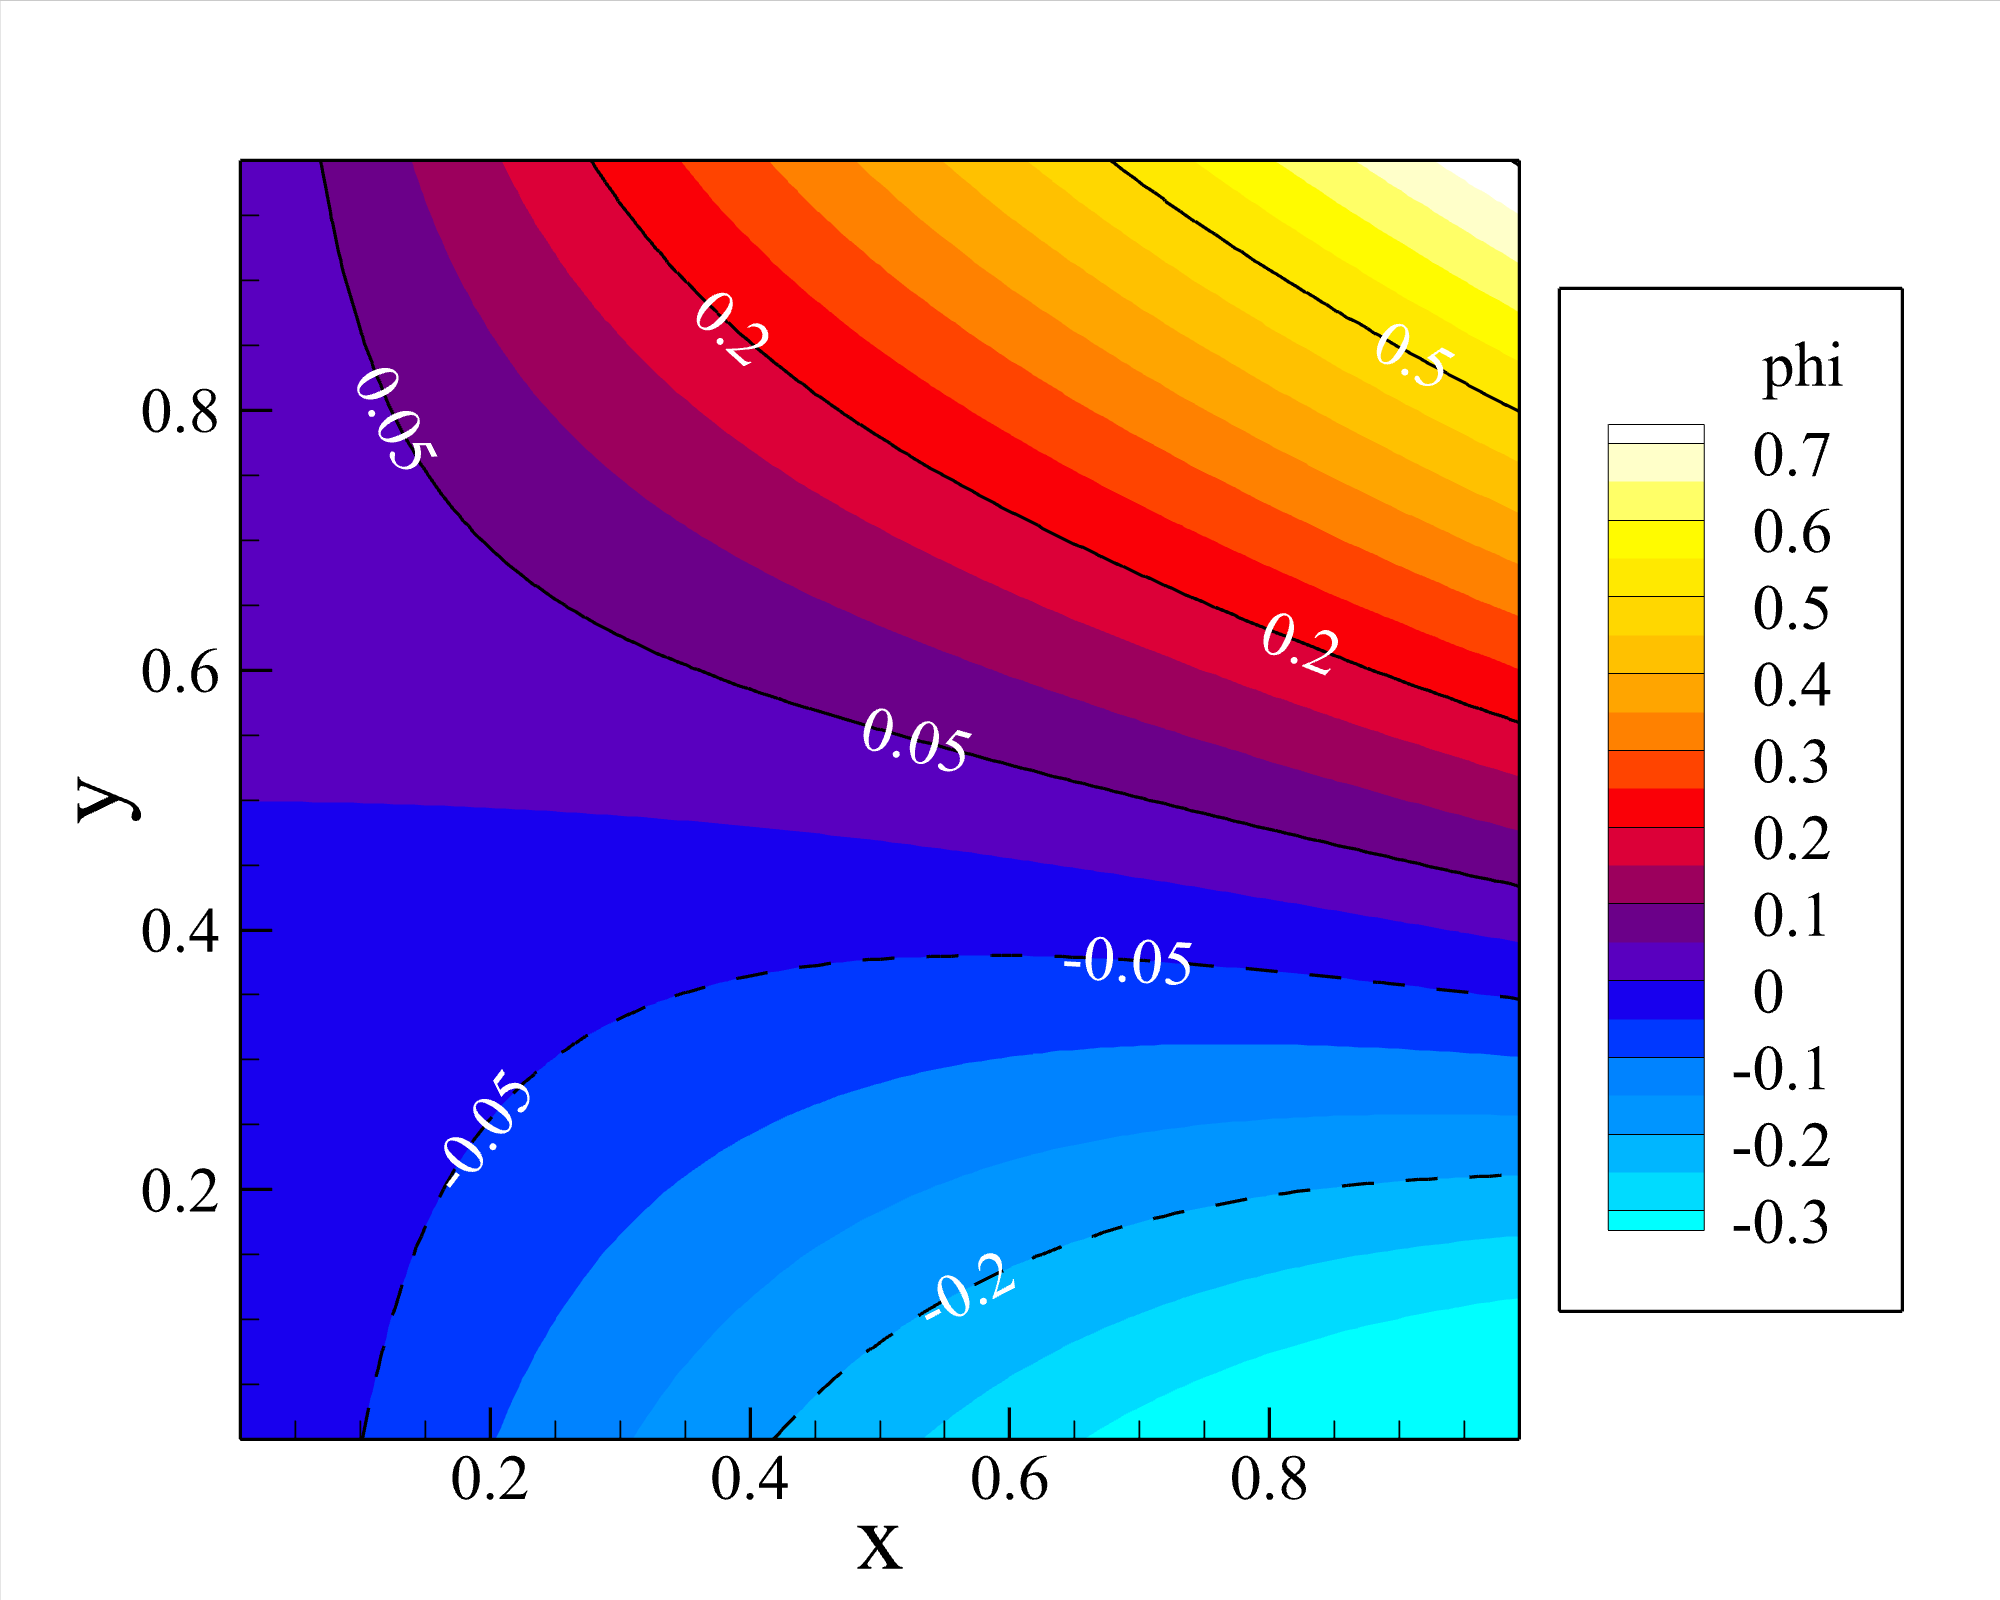
\includegraphics[width=.45\linewidth]{figure/poisson/MG-GS-sol.png}}
	\subfigure[MG-GS 残差分布]{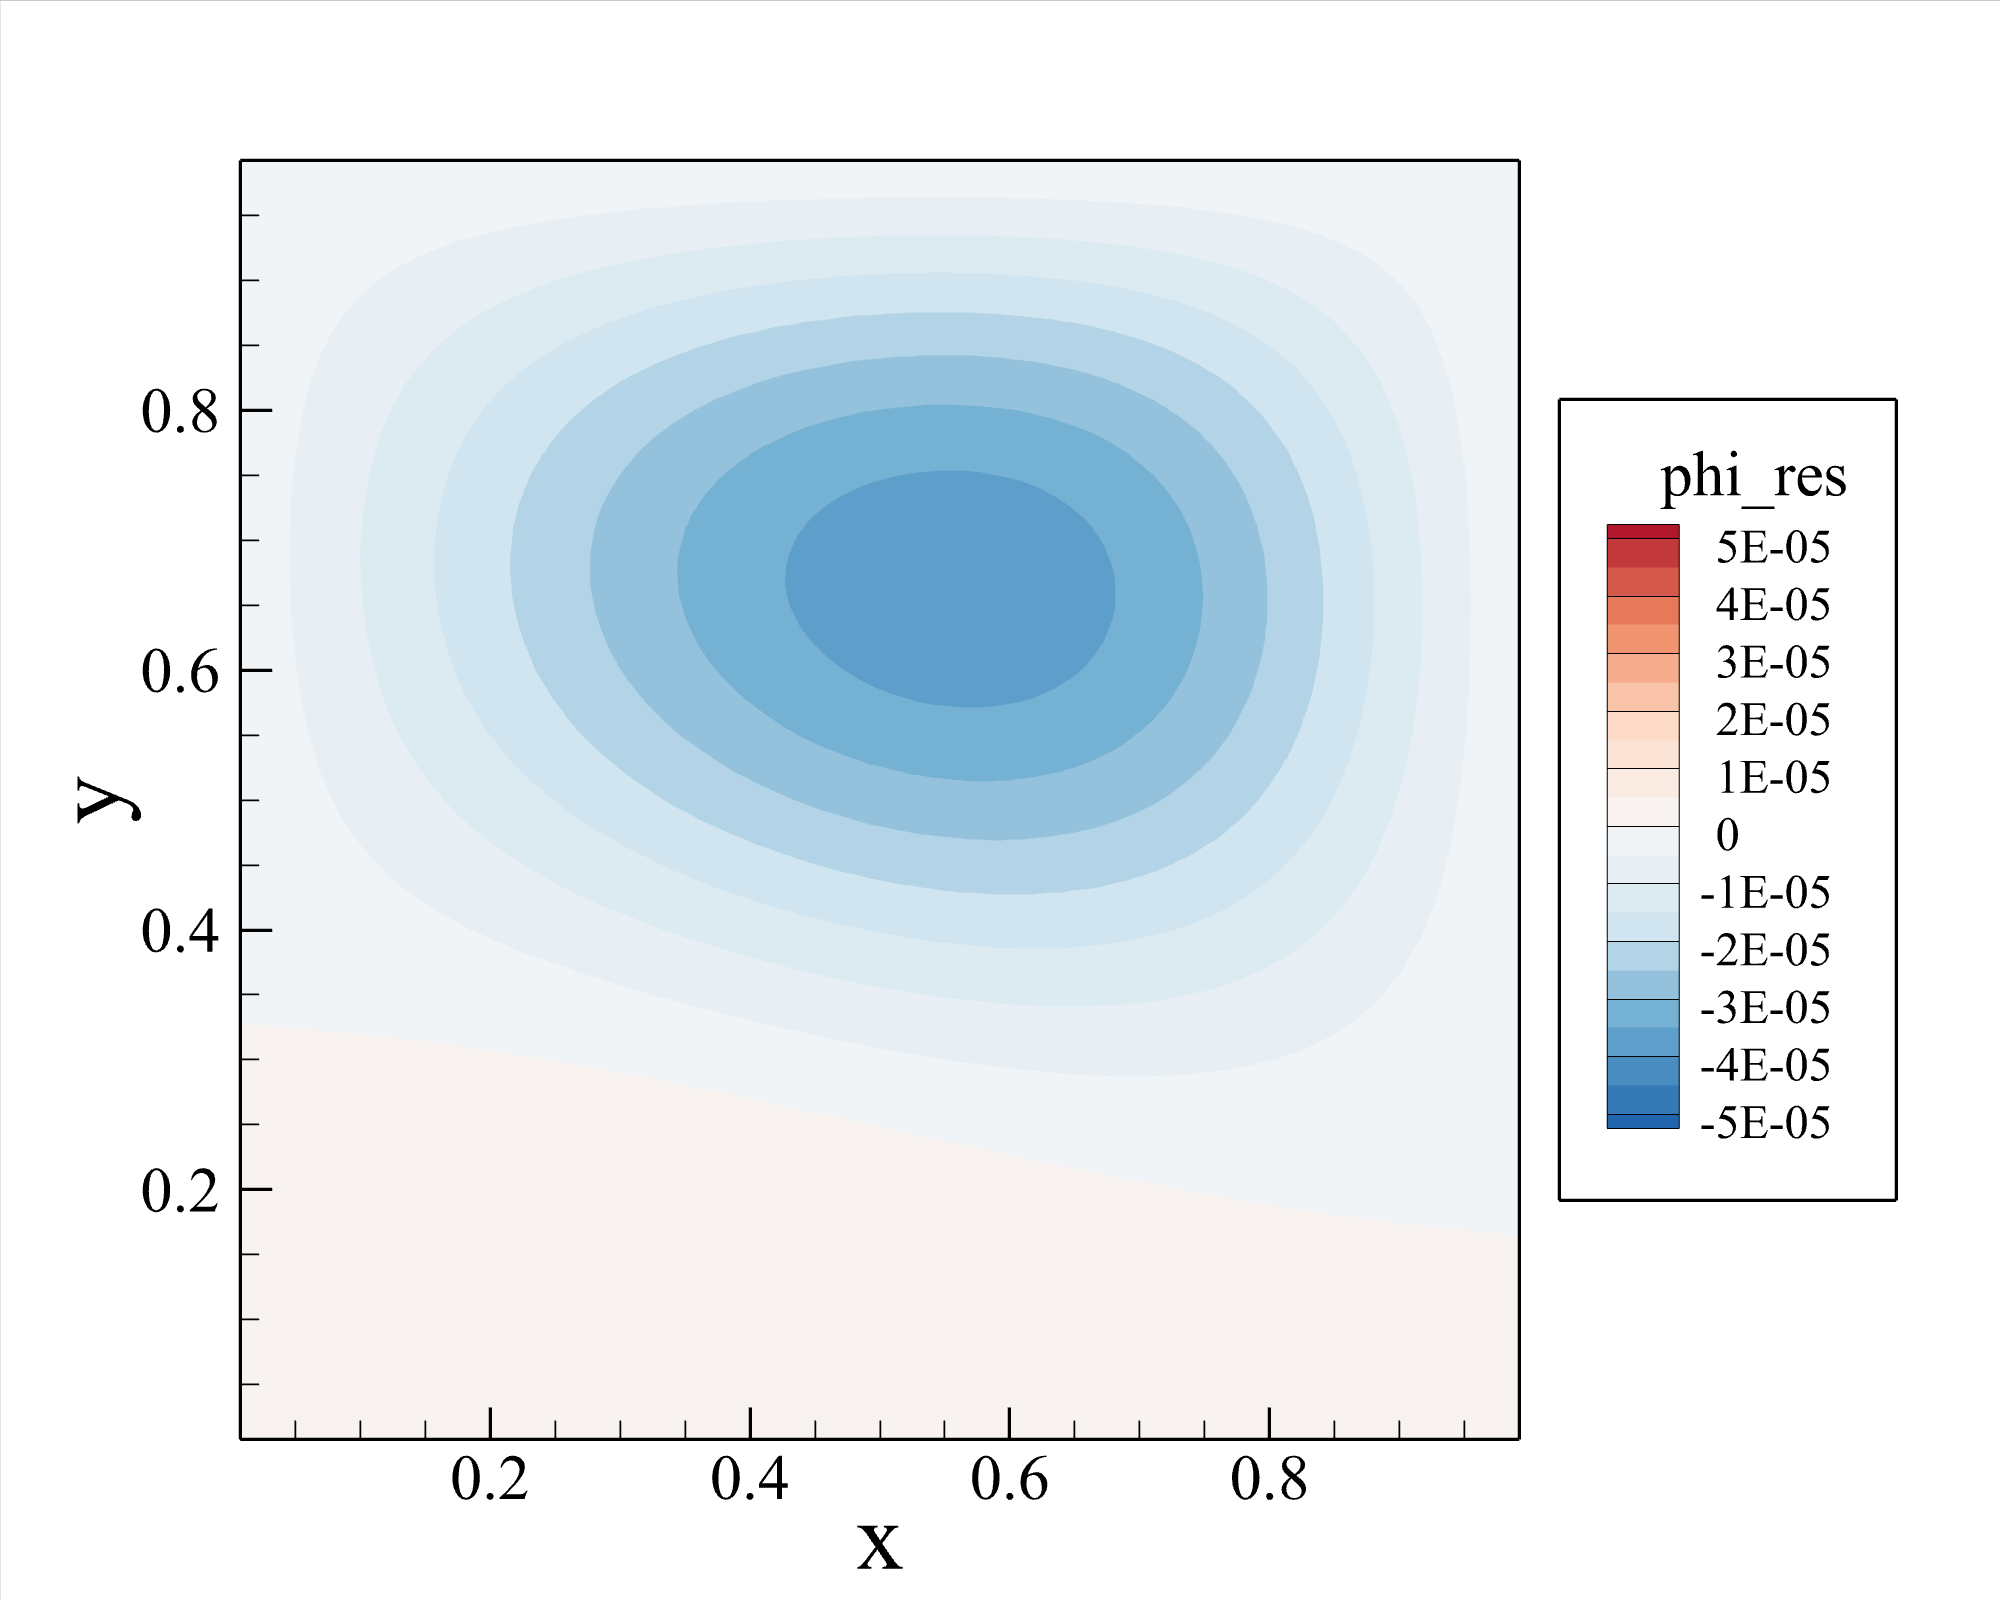
\includegraphics[width=.45\linewidth]{figure/poisson/MG-GS-res.png}}

	\subfigure[MG-SOR 解分布]{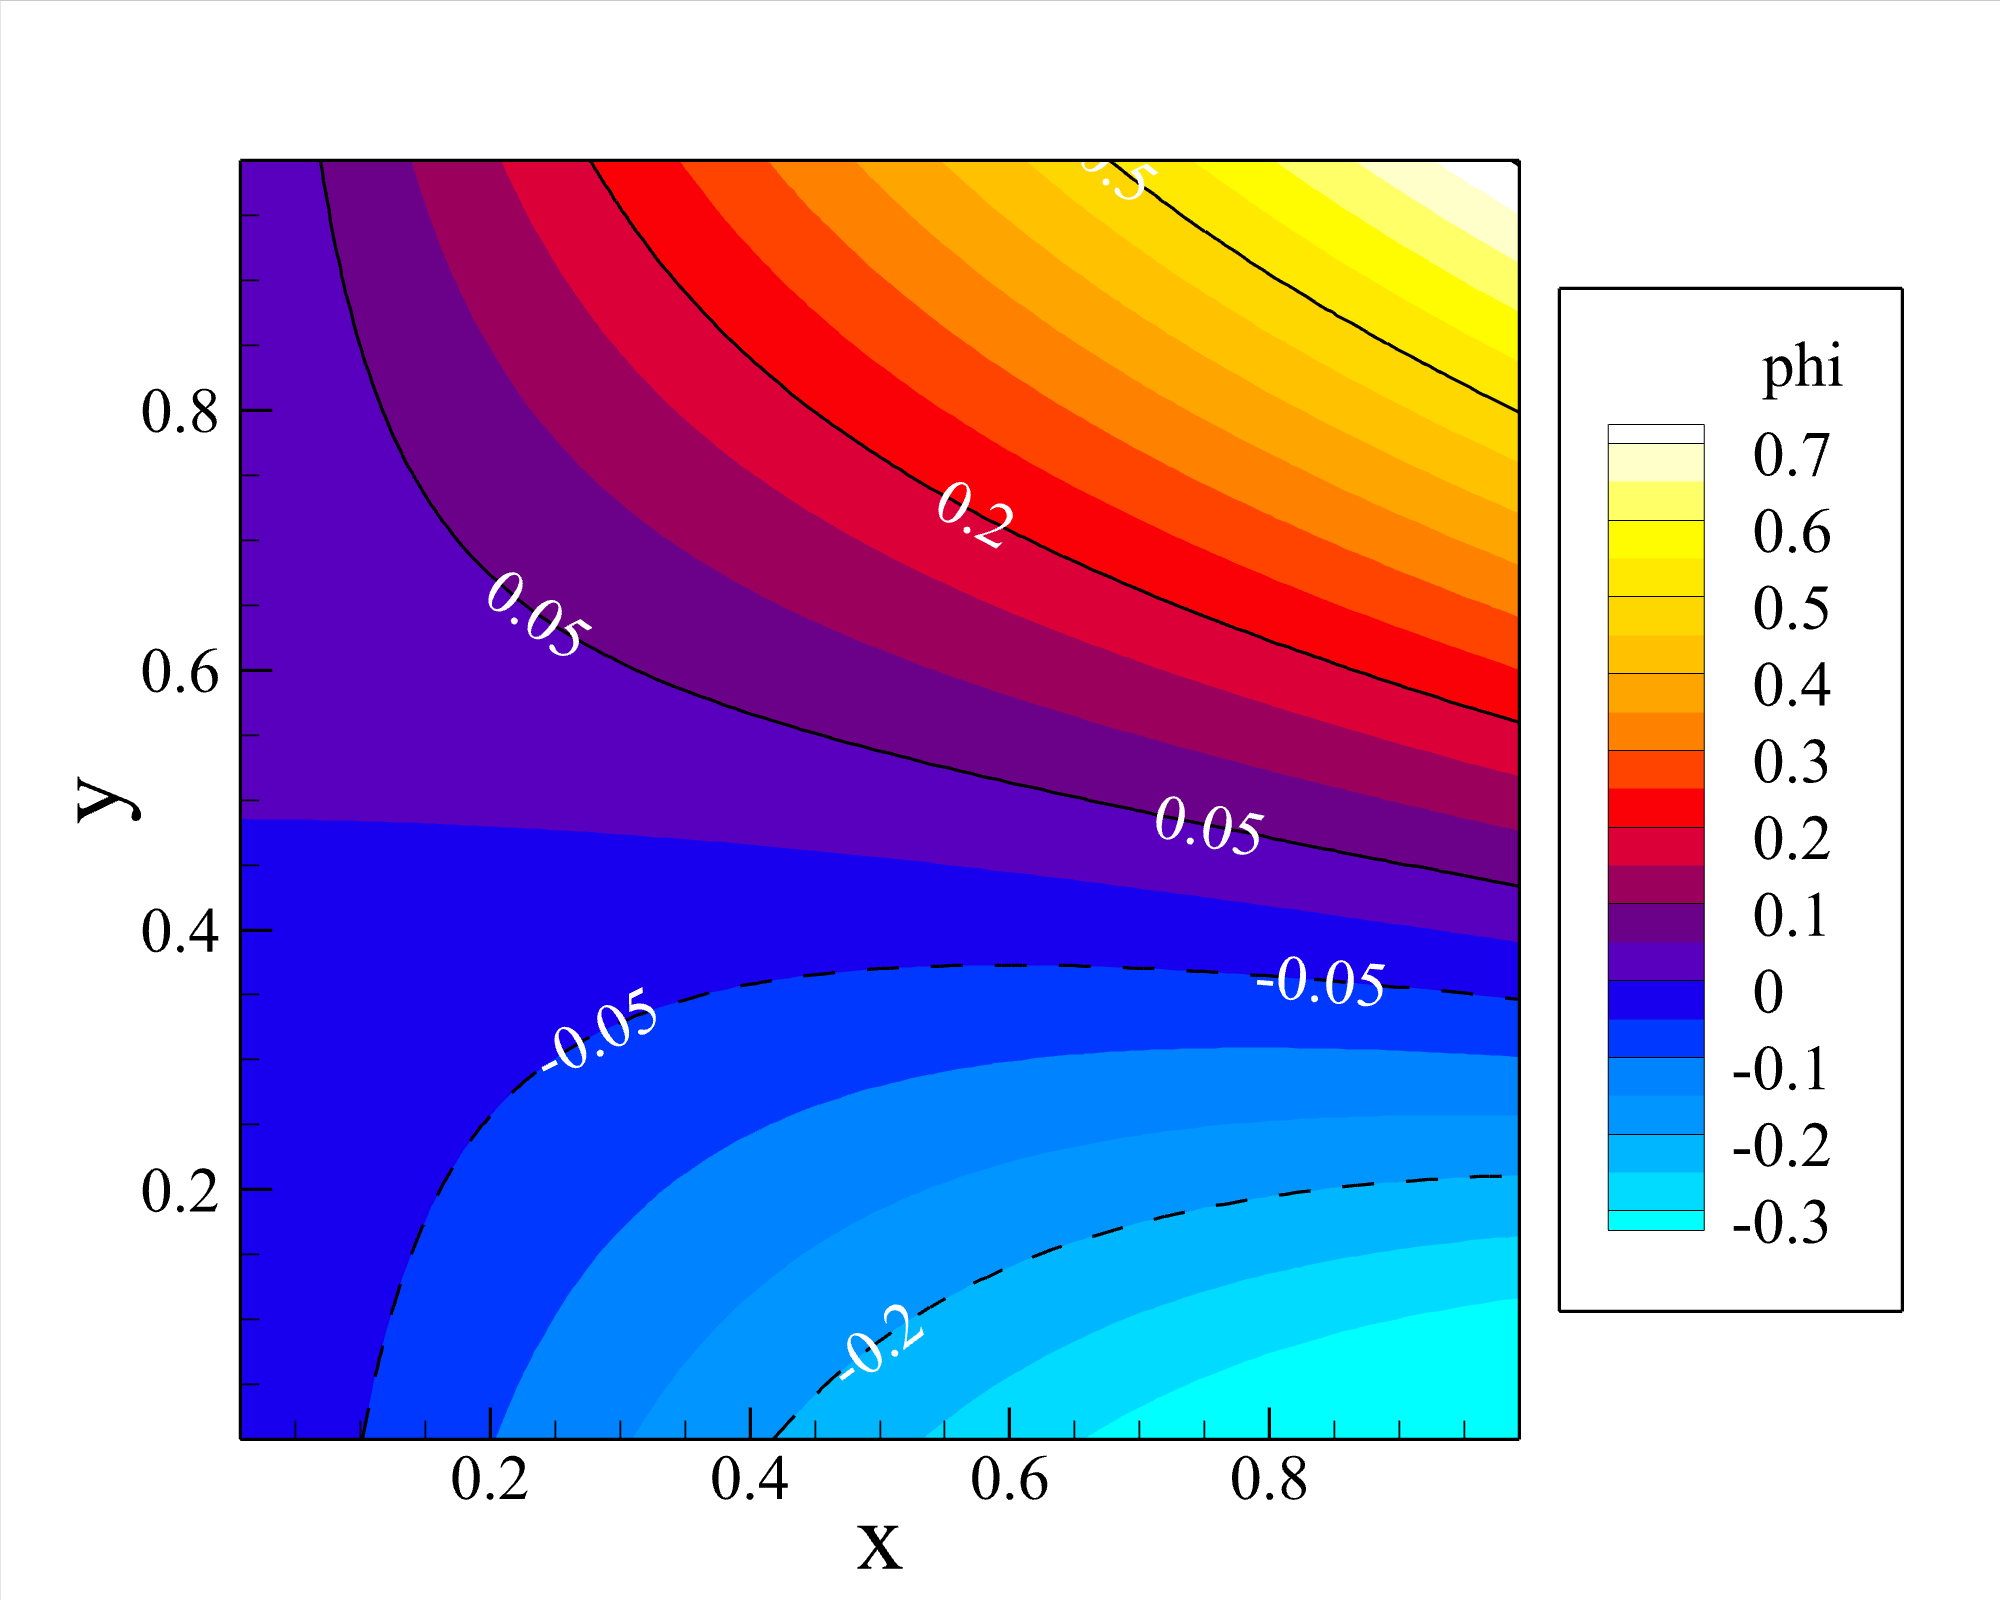
\includegraphics[width=.45\linewidth]{figure/poisson/MG-SOR-sol.png}}
	\subfigure[MG-SOR 残差分布]{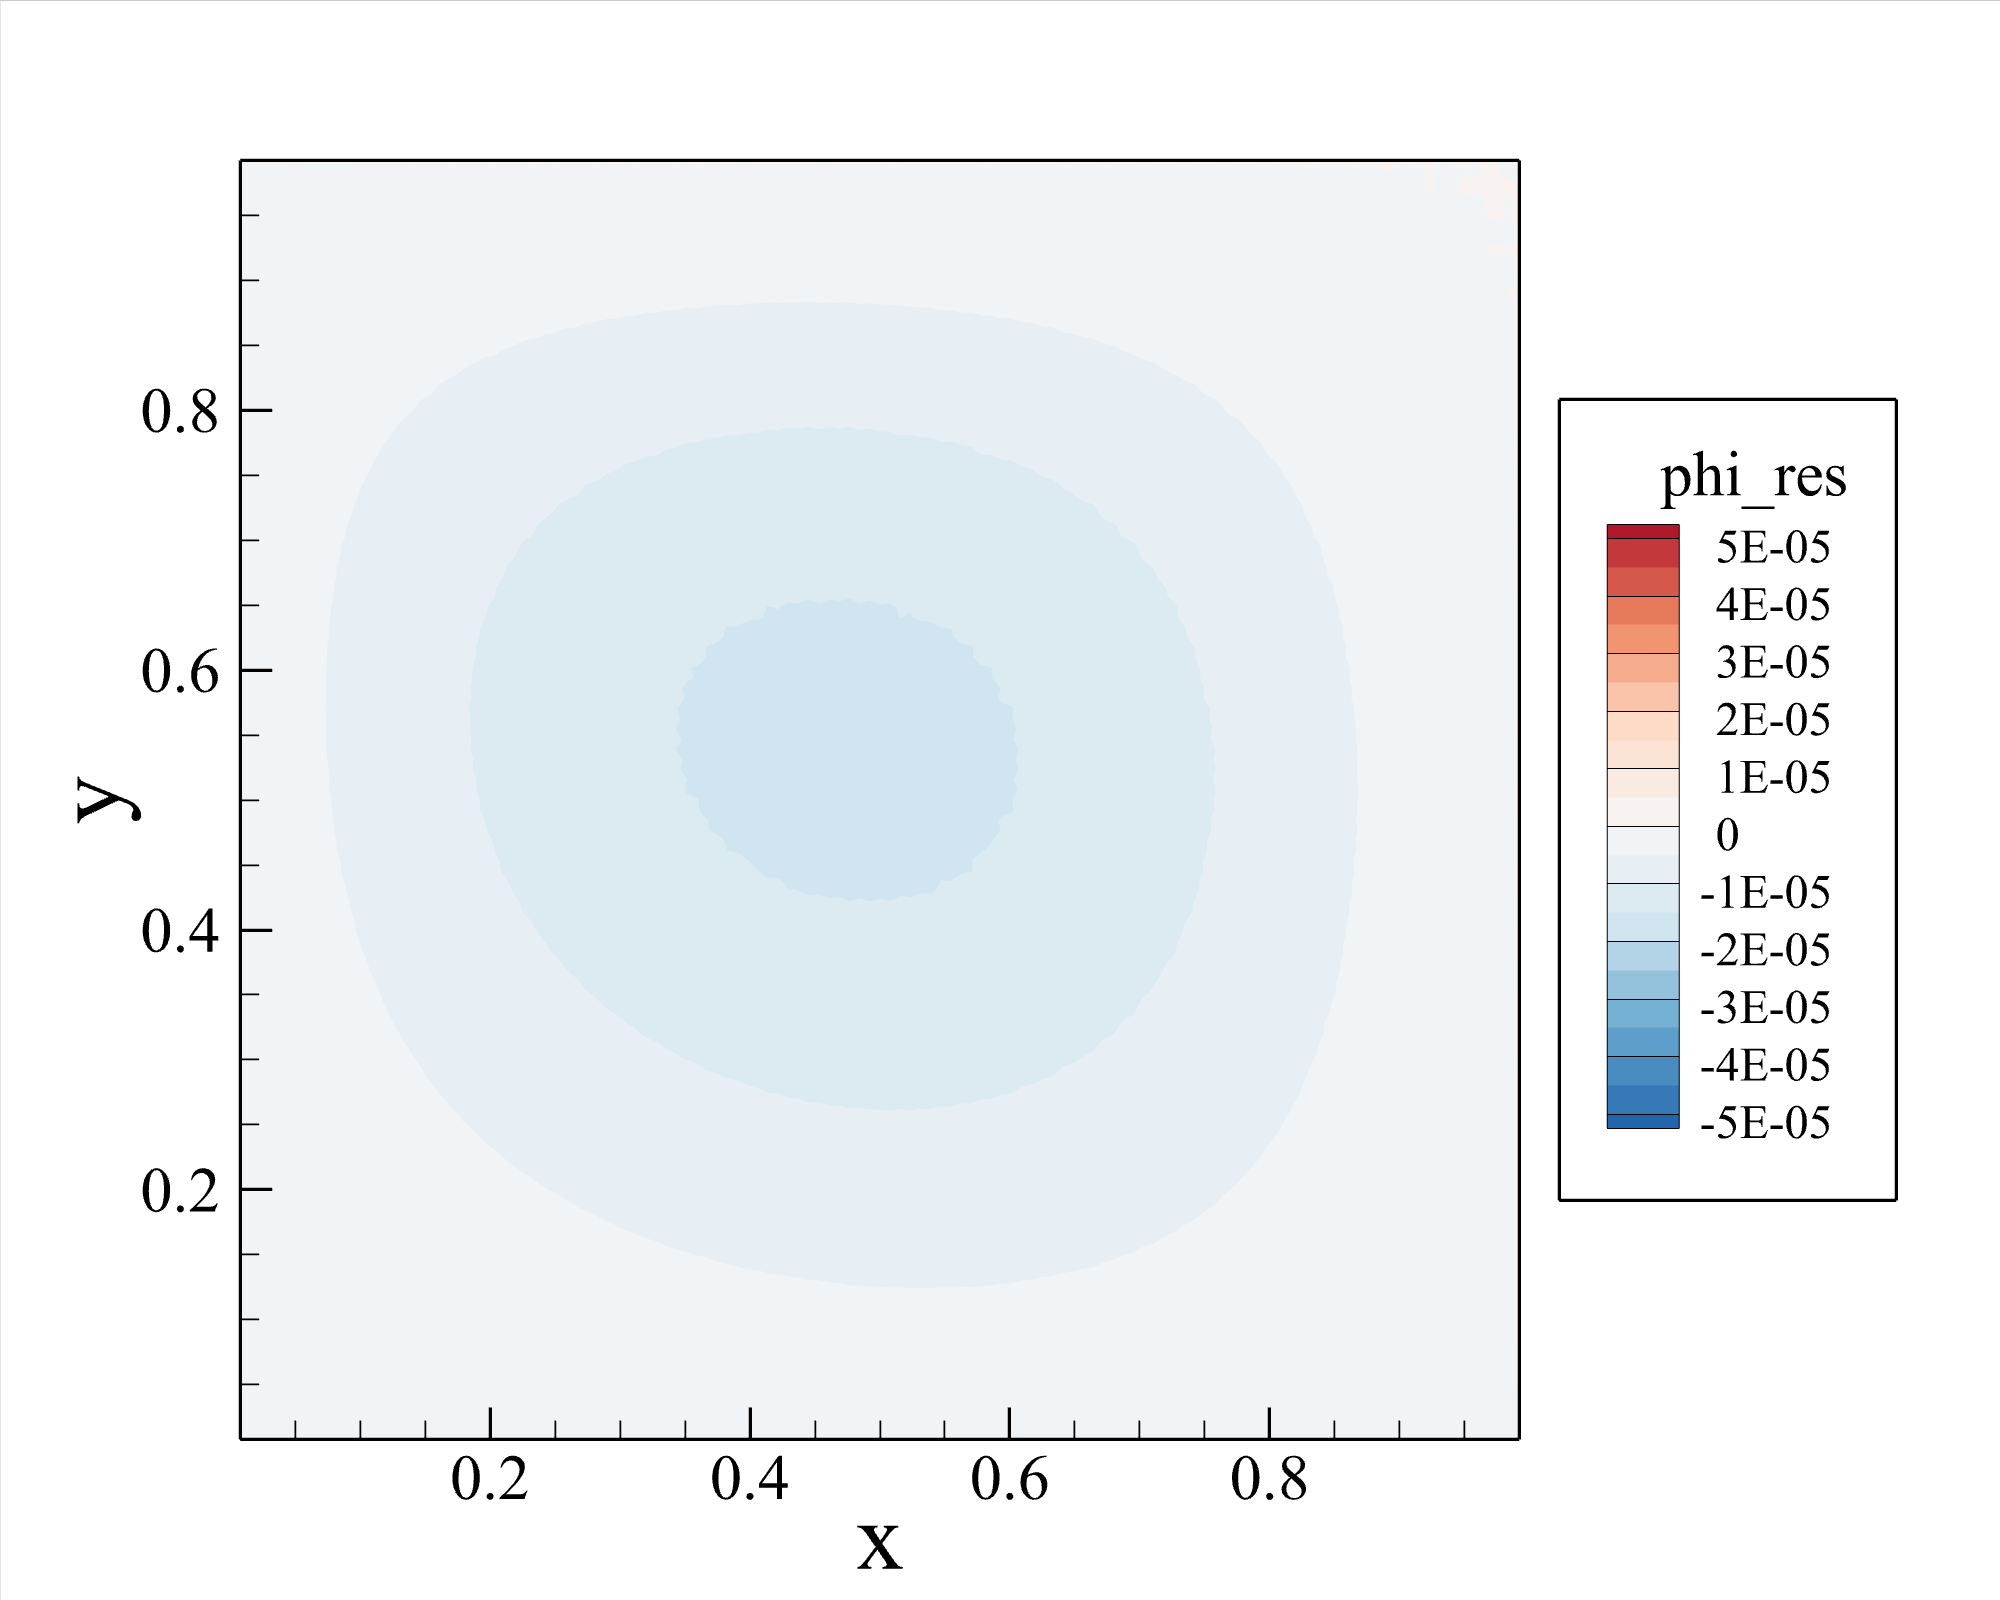
\includegraphics[width=.45\linewidth]{figure/poisson/MG-SOR-res.png}}

	\caption{\label{fig:poisson2}各种迭代法求解Poisson方程的结果与残差}
\end{figure}


\newpage
\section{Sod shock tube problem}
针对如下Sod激波管问题:
\begin{align}
	 & \left\{\begin{array}{l}
		\dfrac{\partial\rho}{\partial t}+\dfrac{\partial(\rho u)}{\partial x}=0         \\[8pt]
		\dfrac{\partial(\rho u)}{\partial t}+\dfrac{\partial(\rho u^2+p)}{\partial x}=0 \\[8pt]
		\dfrac{\partial(\rho E)}{\partial t}+\dfrac{\partial(\rho Eu+pu)}{\partial x}=0
	\end{array}\right.,\quad x\in[0,1] \label{eqn:euler}           \\
	 & \text{IC: }\left(\rho,\ u,\ p\right)|_{t=0}=\left\{\begin{array}{ll}
		(1,\ 0,\ 1)       & x<0.5    \\
		(0.125,\ 0,\ 0.1) & x\geq0.5
	\end{array}\right.
\end{align}
分别采用Lax–Wendroff格式、van Leer格式、Roe格式、5阶WENO格式计算其数值解。

\subsection{Conservation law and Riemann problem}
作为激波管问题以及第三题的理论基础,这里简要介绍一维欧拉方程的黎曼问题,主要参考\citet{toro_riemann_2009}一书。定义守恒律为可写为如下形式的偏微分方程组:
\begin{equation}
	\bm{U}_t+\bm{F}(\bm{U})_x=\bm{0}
\end{equation}
其中
\begin{equation}
	\bm{U}=\left[\begin{matrix}
			u_1    \\
			u_2    \\
			\vdots \\
			u_m
		\end{matrix}\right],\quad
	\bm{F}(\bm{U})=\left[\begin{matrix}
			f_1    \\
			f_2    \\
			\vdots \\
			f_m
		\end{matrix}\right]
\end{equation}
$\bm{U}$称为守恒变量,$\bm{F}(\bm{U})$称为通量矢量,定义Jacobian矩阵为通量函数对守恒变量的偏导(张量)$\bm{A}(\bm{U})\equiv\partial\bm{F}/\partial\bm{U}$。若Jacobian具有$m$个互不相同的实特征值$\lambda_i$(对应$m$个线性无关的特征向量$\bm{K}^{(i)}$),那么该系统被称为双曲守恒律。

\begin{figure}[htbp]
	\centering
	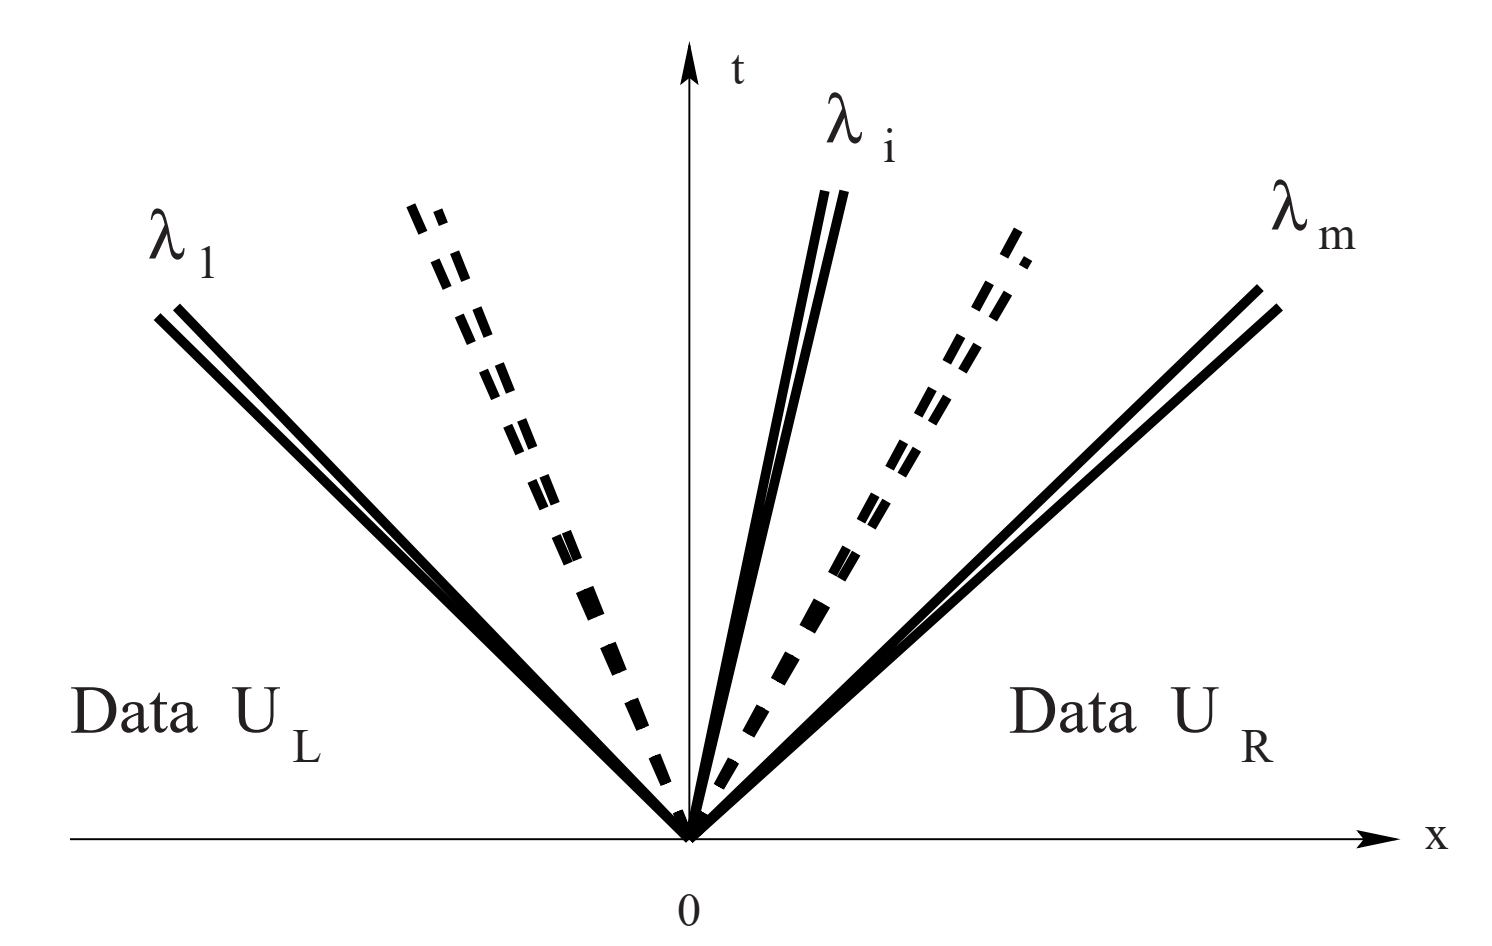
\includegraphics[width=.4\linewidth]{figure/shocktube/riemann.png}
	\caption{\label{fig:riemann}黎曼问题解的结构}
\end{figure}

一般$m\times m$非线性双曲系统的黎曼问题定义为如下初值问题:
\begin{equation}
	\left.\begin{array}{l}
		\bm{U}_t+\bm{F}(\bm{U})_x=\bm{0} \\
		\bm{U}(x,0)=\bm{U}^{(0)}(x)=\left\{\begin{array}{ll}
			\bm{U}_L & \text{if }x<0 \\
			\bm{U}_R & \text{if }x>0
		\end{array}\right.
	\end{array}\right\}
\end{equation}


对于线性系统,黎曼问题的解可以通过叠加原理直接从初值得到。在非线性情况下,根据左右值关系以及特征线方向(特征值),黎曼问题的解由几类基本波(elementary-wave)组成。考虑理想气体的欧拉方程,存在三种基本波:激波、接触间断以及稀疏波(前两者表现为间断,稀疏波表现为由波头、波尾包围的一段连续变化的区域),见\autoref{fig:wave}。


\begin{figure}[htbp]
	\centering
	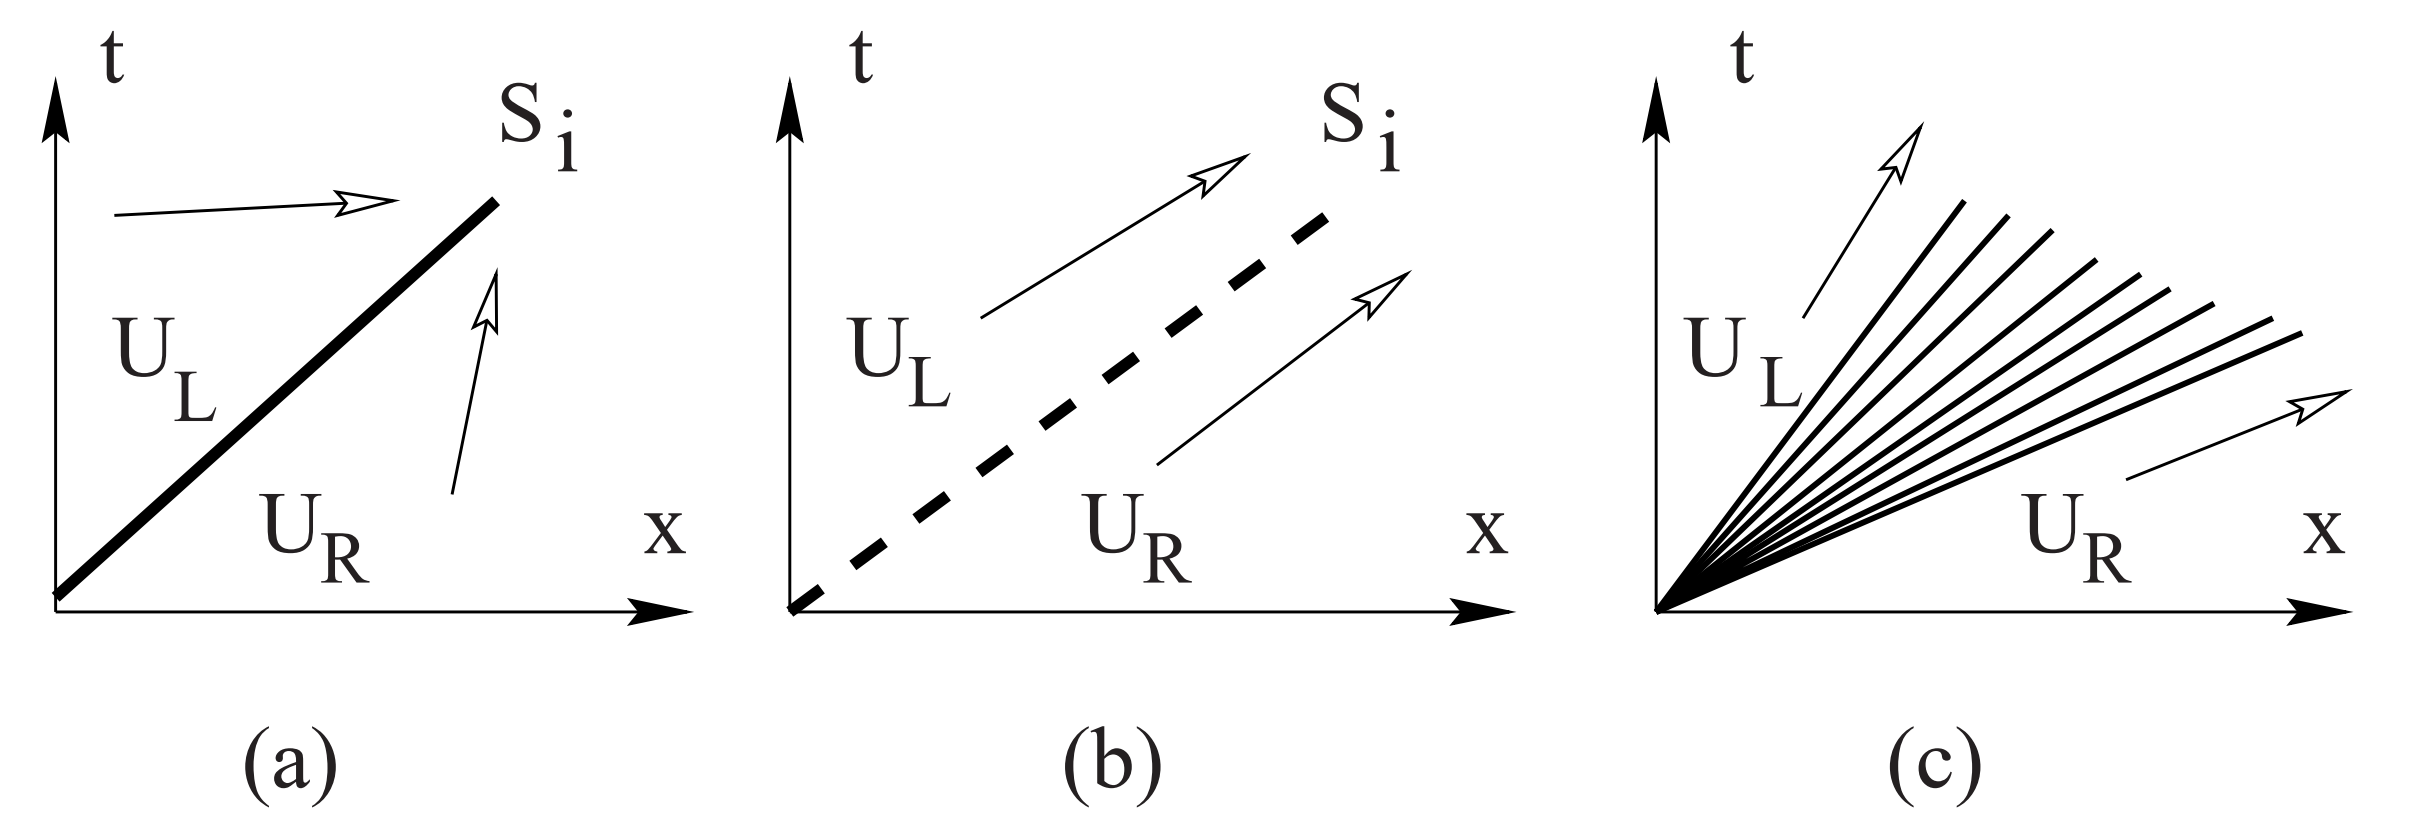
\includegraphics[width=.8\linewidth]{figure/shocktube/wave.png}
	\caption{\label{fig:wave}一维欧拉方程黎曼问题解的三种基本波类型}
\end{figure}

\subsection{The Riemann problem for 1D Euler equations}
考虑一维欧拉方程的守恒形式\footnote{这里$E$表示单位体积总能而非比总能,与题目中的定义不同。}:
\begin{eqnarray}
	\left.
	\begin{array}{l}
		\bm{U}_t+\bm{F}(\bm{U})_x=\bm{0} \\
		\bm{U}=\left[\begin{matrix}
				\rho   \\
				\rho u \\
				E
			\end{matrix}\right]\ ,\quad
		\bm{F}=\left[\begin{matrix}
				\rho u     \\
				\rho u^2+p \\
				u(E+p)
			\end{matrix}\right]
	\end{array}
	\right\}
\end{eqnarray}
黎曼问题的初始条件(间断):
\begin{equation}
	\bm{U}(x,0)=\bm{U}^{(0)}(x)=\left\{\begin{array}{l}
		\bm{U}_L\quad \text{if }x<0 \\
		\bm{U}_R\quad \text{if }x>0
	\end{array}\right.
\end{equation}
上式为欧拉方程的守恒形式,$E=\frac{p}{\gamma-1}+\frac{1}{2}\rho u^2$为单位体积总能。

该问题解的一般结构如\autoref{fig:euler}所示。通常由左行波、接触间断以及一道右行波组成,分别对应系统的三个特征值($u-a,\ u,\ u+a$),其中行波可以是稀疏波和激波两种。两道行波将$x-t$空间划分为三个区域:L区、*区和R区,其中*区进一步被接触间断划分为*L和*R两部分,*L和*R区速度、压力相同,但密度不同。
\begin{figure}[htbp]
	\centering
	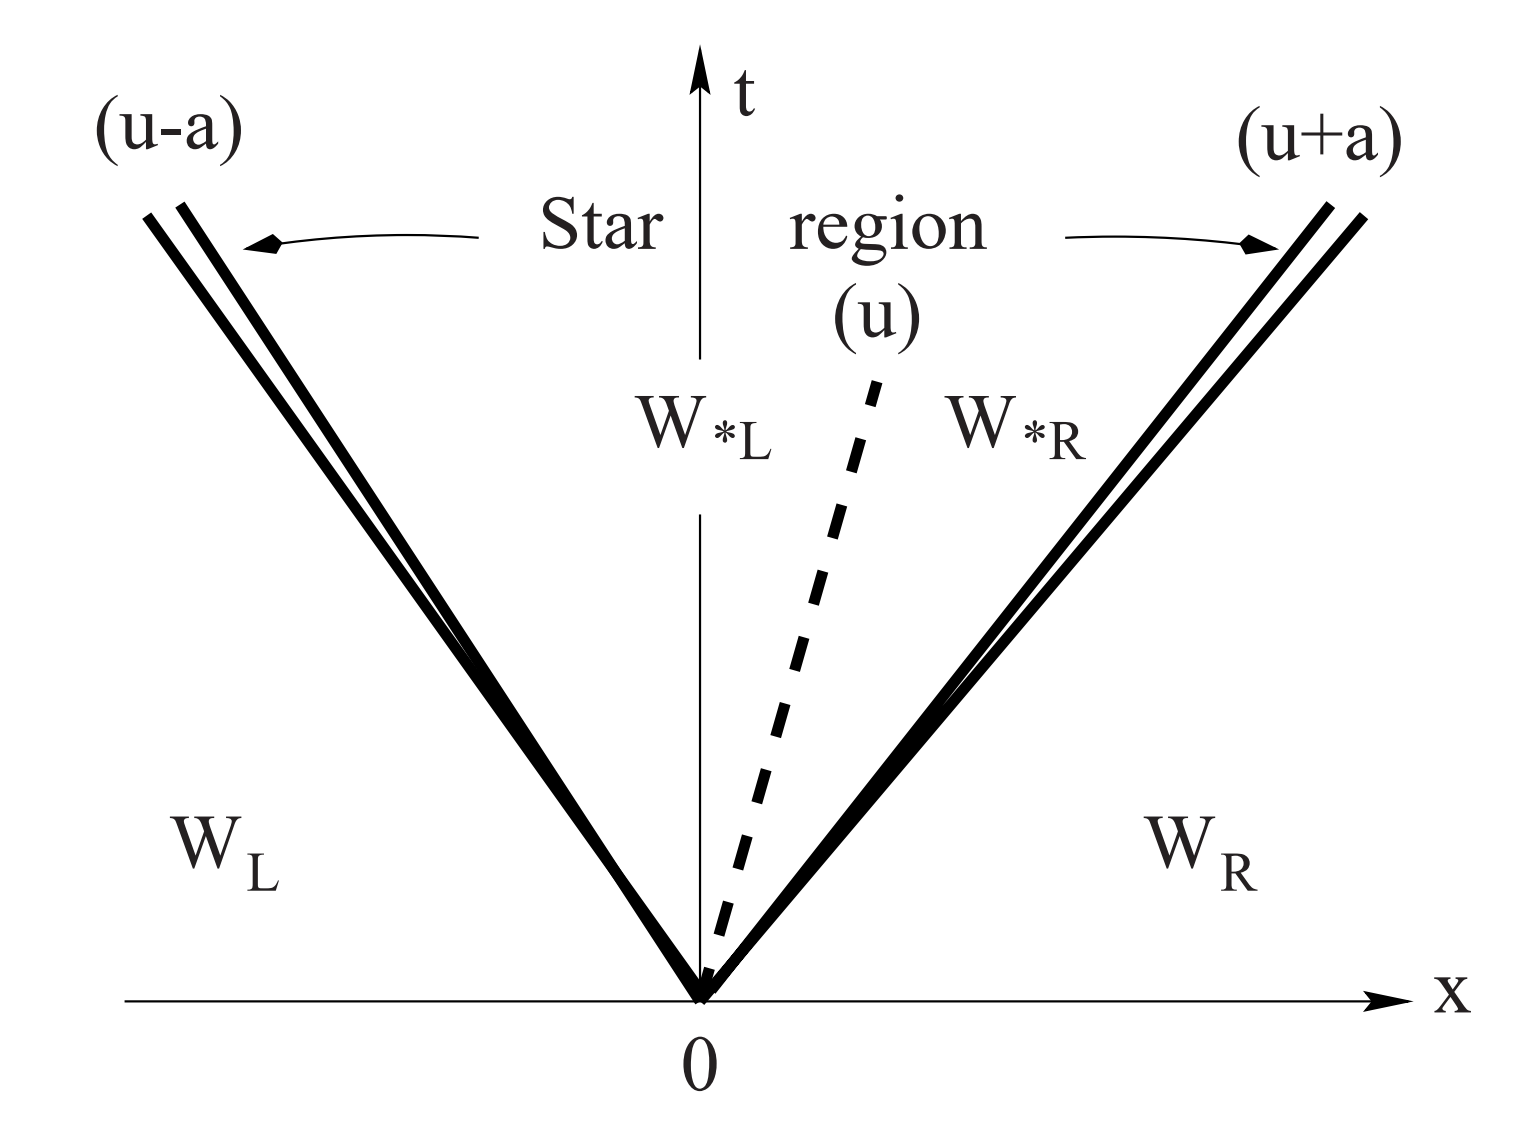
\includegraphics[width=.4\linewidth]{figure/shocktube/euler.png}
	\caption{\label{fig:euler}一维欧拉方程黎曼问题解的一般形式}
\end{figure}

一维欧拉方程的黎曼问题精确解由初始间断左右参数$\bm{U}_{L,R}$唯一确定,其求解思路是先基于左右值判断左右行波类型、得到*区参数,随后根据激波、稀疏波关系得到全空间的精确解。*区压强和速度由下式\footnote{实际上就是稀疏波(等熵流)、激波(Rankine–Hugoniot条件)的压强匹配关系。}给出:
\begin{eqnarray}
	f(p,\bm{W}_L,\bm{W}_R)=f_L(p,\bm{W}_L)+f_R(p,\bm{W}_R)+\Delta u=0,\ \Delta u\equiv u_R-u_L, \\
	u_*=\frac{1}{2}(u_L+u_R)+\frac{1}{2}\left[f_R(p_*)-f_L(p_*)\right]
\end{eqnarray}
这里$\bm{W}$表示原始变量$(\rho,\ u,\ p)^T$,上式种压强函数具体形式为:
\begin{equation}
	f_L(p_L,\bm{W}_L)=\left\{\begin{array}{ll}
		(p-p_L)\left[\frac{A_L}{p+B_L}\right]^{\frac{1}{2}}                                               & \text{if }p>p_L\text{ (shock)}           \\
		\frac{2a_L}{(\gamma_L-1)}\left[\left(\frac{p}{p_L}\right)^{\frac{\gamma_L-1}{2\gamma_L}}-1\right] & \text{if }p\leq p_L\text{ (rarefaction)}
	\end{array}\right.
\end{equation}
\begin{equation}
	f_R(p_R,\bm{W}_R)=\left\{\begin{array}{ll}
		(p-p_R)\left[\frac{A_R}{p+B_R}\right]^{\frac{1}{2}}                                               & \text{if }p>p_R\text{ (shock)}           \\
		\frac{2a_R}{(\gamma_R-1)}\left[\left(\frac{p}{p_R}\right)^{\frac{\gamma_R-1}{2\gamma_R}}-1\right] & \text{if }p\leq p_R\text{ (rarefaction)}
	\end{array}\right.
\end{equation}
其中常系数为:
\begin{eqnarray}
	\left.\begin{array}{l}
		A_L=\frac{2}{(\gamma_L+1)\rho_L},\ B_L=\frac{\gamma_L-1}{\gamma_L+1}p_L, \\
		A_R=\frac{2}{(\gamma_R+1)\rho_R},\ B_R=\frac{\gamma_R-1}{\gamma_R+1}p_R, \\
	\end{array}\right\}
\end{eqnarray}
数值上利用Newton-Raphson迭代即可求解上述压力方程,该黎曼问题解具有自相似特性,即变量的值仅依赖于$s\equiv x/t$,基于判断得到的左右行波类型,可以由稀疏波、激波关系采样得到各变量在$(x,t)$的值。

\subsection{Lax-Wendroff scheme}
Lax-Wendroff格式是一类具有时/空间两阶精度的双曲型偏微分方程有限差分格式。包含预估、校正的两步Lax-Wendroff格式如下所示:
\begin{equation}
	\left\{\begin{array}{ll}
		\text{Step 1: prediction} & \bm{U}_{j+\frac{1}{2}}^*=\dfrac{1}{2}\left(\bm{U}_j^n+\bm{U}_{j+1}^n\right)-\dfrac{\Delta t}{2\Delta x}\left[\bm{F}(\bm{U}_{j+1}^n)-\bm{F}(\bm{U}_{j}^n)\right] \\[6pt]
		\text{Step 2: correction} & \bm{U}_j^{n+1}=\bm{U}_j^n-\dfrac{\Delta t}{\Delta x}\left[\bm{F}(\bm{U}_{j+1}^*)-\bm{F}(\bm{U}_{j}^*)\right]
	\end{array}\right.
\end{equation}

\subsection{Shock capturing}
数值求解非线性双曲型偏微分方程中,最关键的问题就是激波(间断)的捕捉,其中核心思路就是要根据物理上信息传播的方向来确定离散格式的构造,否则会出现非物理振荡,甚至计算发散。目前有两类数值方法可以实现迎风方向(即信息传播方向)的识别:
\begin{enumerate}[label=(\arabic*)]
	\item 通量矢量分裂,Flux vector splitting (FVS);
	\item 通量差分分裂,Flux difference splitting (FDS),也称Godunov类方法。
\end{enumerate}

前者可以看作是有限差分方法中一阶迎风格式的理论拓展,通过双曲守恒律中系数矩阵特征值判断波传播方向,将通量拆分为正负两个方向的部分,分别迎风插值近似。典型通量分裂格式包括Lax-Friedrichs splitting、Steger-Warming splitting、van Leer splitting、Liou-Steffen splitting (也称AUSM格式)。

后者则采取了截然不同的方法论(Godunov思想,有限体积法),即将已知的变量离散分布,看作其在空间中划分出的控制体上的分片平均,通过求解各控制体边界上的局部黎曼问题,得到全流场的解。局部黎曼问题可以采用精确黎曼求解器求解,但计算量极大且并不会体现出精度优势;更常见的方法是使用近似黎曼求解器,包括近似状态黎曼求解器(假定左右行波类型)、HLL/HLLC黎曼求解器(基于两波、三波近似)、Roe黎曼求解器(求解局部线化问题)等。

\subsection{Flux vector splitting methods}
对于守恒律,时间上保持连续形式,空间上离散化:
\begin{equation}
	\frac{\mathrm{d}\bm{U}_i}{\mathrm{d}t}=-\frac{\Delta t}{\Delta x}\left(\bm{F}_{i+\frac{1}{2}}-\bm{F}_{i-\frac{1}{2}}\right)
\end{equation}
其中数值通量拆分为:
\begin{equation}
	\bm{F}_{i+\frac{1}{2}}=\bm{F}_i^+(\bm{U}_i^n)+\bm{F}_{i+1}^-(\bm{U}_{i+1}^n)
\end{equation}
分别表示沿$x$正向与负向传播的部分对边界处通量的贡献。分裂通量的具体形式取决于对系数矩阵特征值$\lambda=\lambda^++\lambda^-$的分裂方法。记$\bm{\Lambda}^{\pm}\equiv\mathrm{diag}\left(\lambda_1^\pm,\cdots \lambda_m^\pm\right)$,$\bm{K}$为对应特征向量构成的矩阵,于是有:
\begin{equation}
	\bm{F}^\pm=\bm{A}^\pm\bm{U}=\bm{K}^{-1}\bm{\Lambda}^\pm\bm{K}\bm{U}
\end{equation}

一维欧拉方程系数矩阵特征值为$(\lambda_1,\lambda_2,\lambda_3)=(u-a,\ u,\ u+a)$,其中$a=\sqrt{\gamma p/\rho}$为声速。

\subsubsection{Steger-Warming splitting}
若特征值按如下方式分裂:
\begin{equation}
	\lambda_i^+=\frac{1}{2}(\lambda_i+|\lambda_i|),\quad\lambda_i^-=\frac{1}{2}(\lambda_i-|\lambda_i|)
\end{equation}
那么可以得到Steger-Warming通量矢量分裂格式,分裂通量为:
\begin{equation}
	\bm{F}^\pm=\frac{\rho}{2\gamma}\left[\begin{matrix}
			\lambda_1^\pm+2(\gamma-1)\lambda_2^\pm+\lambda_3^\pm            \\
			(u-a)\lambda_1^\pm+2(\gamma-1)u\lambda_2^\pm+(u+a)\lambda_3^\pm \\
			(H-ua)\lambda_1^\pm+(\gamma-1)u^2\lambda_2^\pm+(H+ua)\lambda_3^\pm
		\end{matrix}\right]
\end{equation}
其中$H=(E+p)/\rho$为总比焓。

\subsubsection{Van Leer splitting}
Van Leer在构造通量分裂时额外增加了两项条件:
\begin{enumerate}[label=(\arabic*)]
	\item 分裂Jacobian矩阵$\bm{A}^\pm=\frac{\partial\bm{F}^\pm}{\partial\bm{U}}$是连续的;
	\item 分裂通量可以退化为亚声速流。
\end{enumerate}
其分裂通量为:
\begin{equation}
	\bm{F}^\pm=\pm\dfrac{1}{4}\rho a(1\pm M)^2\left[\begin{matrix}
			1                                                        \\
			\dfrac{2a}{\gamma}\left(\dfrac{\gamma-1}{2}M\pm 1\right) \\
			\dfrac{2a^2}{\gamma^2-1}\left(\dfrac{\gamma-1}{2}M\pm 1\right)^2
		\end{matrix}\right]
\end{equation}
其中$M=u/a$为马赫数。

\subsection{Flux difference splitting methods}
\subsubsection{Roe-Pike method}
不同于近似状态黎曼求解器近似行波类型,HLL/HLLC黎曼求解器近似解的结构,Roe方法的思路在于直接将系统方程(非线性双曲守恒律)做线性近似,进而得到边界上通量的表达式(无需判断波的类型或速度),因此Roe方法在CFD等领域取得了广泛的应用。

原始Roe方法需要构造平均Jacobian矩阵,事实上该构造过程是没有必要的,Roe,Pike提出了另一种实现方法,避免了矩阵运算。

\subsection{High order methods}
前文介绍的方法仅告诉我们如何确定信息传播方向,避免间断附近的非物理振荡,插值过程直接采用一阶精度迎风格式。但在实际可压缩流动数值模拟中,我们还需要通过提高插值格式的阶数来提高离散解的精度,对于存在间断的流场,插值格式也需要特殊的构造以实现“激波捕捉”这一特性。

\subsubsection{WENO reconstruction}
加权本质无振荡(weighted essentially non-oscillatory, WENO)格式\citep{liu_weighted_1994}是在本质无振荡(ENO)格式思想上的进一步拓展,根据子模版上的光滑程度对插值结果加权,而非ENO方法中仅保留最光滑的模板。\citet{jiang_efficient_1996}一文在最初版本WENO的基础上提出了一种新的光滑因子计算方法,这一形式的WENO格式也称WENO-JS,在流体力学等领域取得了极为广泛的应用。

接下来我们对ENO/WENO方法中最基本的思想和操作步骤简单做一个简单的介绍:
\paragraph{重构} 对于双曲守恒律,将离散节点上的值看作单个网格内的平均值(即有限体积思想)
\begin{equation}
	\bar{v}_i\equiv\frac{1}{\Delta x_i}\int_{x_{i-\frac{1}{2}}}^{x_{i+\frac{1}{2}}}v(\xi)\mathrm{d}\xi
\end{equation}
我们通过选取模板(stencil)$S(i)\equiv\{I_{i-r,\cdots,I_{i+s}}\},\ I_i\equiv\left[x_{i-\frac{1}{2}},x_{i+\frac{1}{2}}\right]$,其中$r$表示模板相对$i$节点向左的偏移量。根据模板点上已知的平均值$\bar{v}_{i-r+j},\ j=0,\cdots k-1$做插值,近似$v(x)$的原函数(primitive function)而非其本身:
\begin{equation}
	V(x)\equiv\int_{-\infty}^x v(\xi)\mathrm{d}\xi
\end{equation}
进而间接得到$v$在界面(cell boundary)处的重构值:
\begin{equation}
	v_{i+\frac{1}{2}}=\sum_{j=0}^{k-1}c_{rj}\bar{v}_{i-r+j}
\end{equation}

对于均匀网格$\Delta x_i=\Delta x$,插值系数可由下式求得:
\begin{equation}
	c_{rj}=\sum_{m=j+1}^k\dfrac{\sum_{l=0;\ l\neq m}^k\prod_{q=0;\ q\neq m,l}^k\left(r-q+1\right)}{\prod_{l=0;\ l\neq m}^k\left(m-l\right)}
\end{equation}
下文所述的ENO、WENO重构都是基于这一插值重构过程,主要区别在于模板的选取方法不同。

\paragraph{ENO重构} 我们知道在牛顿插值中,利用差商(Divided differences)的性质,每增加一个模板点,仅需在原有多项式基础上增添一项,便可得到更高一阶的插值多项式\citep{sauer_numerical_2018}。另一个关键要素在于,差商的大小本身可以表征该模板上值的光滑程度\citep{cockburn_advanced_1998}。

ENO重构的核心思路就是,利用牛顿差商的性质,我们可以从单点模板开始,逐步从左或右扩展模板,每次对比左右扩展模板的光滑程度,选取较光滑的一侧作为高一阶的模板。重复这一模板选取过程,直至达到我们给定的阶数,即可获得当前阶数下光滑程度最好的模板(避开强间断),用于前述重构过程。

\paragraph{WENO重构} 虽然ENO针对双曲守恒律提出了根据光滑程度选取模板的思想,但容易发现上述实现存在许多缺陷:
\begin{enumerate}
	\item 在光滑区间,ENO非必要地舍弃了相对“非光滑”的模板,造成了精度损失;
	\item 数值通量非光滑,即相邻两点间的模板选取可能有明显区别;
	\item 模板选取过程中总共需要考虑$k$个候选模板,覆盖了$2k-1$个网格点,但仅有一个模板被用于最后的重构$k$阶精度;
	\item 模板选取过程中存在大量逻辑运算(if语句),对于早期计算机来说比较耗时。
\end{enumerate}
由此,WENO方法即在ENO思想的基础上提出了按模板光滑程度加权的操作,直接考虑$k$个子模版(无需像ENO一样逐步比较扩展):
\begin{equation}
	S_r(i)=\left\{x_{i-r},\cdots,x_{i-r+k-1}\right\},\quad r=0,\cdots,k-1
\end{equation}
在每个候选模板上,都可以得到$v_{i+\frac{1}{2}}$的重构值:
\begin{equation}
	v_{i+\frac{1}{2}}^{(r)}=\sum_{j=0}^{k-1}c_{rj}\bar{v}_{i-r+j},\quad r=0,\cdots,k-1
\end{equation}
WENO采用了上述子模版重构值的凸组合(convex combination)作为$v(x_{i+\frac{1}{2}})$的近似:
\begin{equation}
	v_{i+\frac{1}{2}}=\sum_{r=0}^{k-1}\omega_rv_{i+\frac{1}{2}}^{(r)}
\end{equation}
其中权重满足$\omega_r\geq0,\ \sum_{r=0}^{k-1}\omega_r=1$。

注意到当所有子模版上函数$v(x)$都光滑的情况下,存在理想权重$d_r$使得上述重构具有$2k-1$阶精度:
\begin{equation}
	v_{i+\frac{1}{2}}=\sum_{r=0}^{k-1}d_r v_{i+\frac{1}{2}}^{(r)}=v(x_{i+\frac{1}{2}})+\mathcal{O}(\Delta x^{2k-1})
\end{equation}
其中$d_r$可以通过对比子模版和全模板(即$2k-1$点构成的整个模板)上多项式重构的系数,求解代数方程组得到。显然,权函数$\omega_r$的设计需要满足在光滑条件下退化为理想权重$d_r$,即$\omega_r=d_r+\mathcal{O}(\Delta x^{2k-1})$。

通过对误差量级的分析以及权函数需满足的稳定性、一致性条件,可以得到下述表达式:
\begin{equation}
	\omega_r=\frac{\alpha_r}{\sum_{s=0}^{k-1}\alpha_s},\quad r=0,\cdots,k-1
\end{equation}
其中:
\begin{equation}
	\alpha_r=\frac{d_r}{(\epsilon+\beta_r)^2}
\end{equation}
\citet{jiang_efficient_1996}提出了光滑因子(smooth indicators)$\beta_r$的一种形式(与基于$L^1$模的总变差定义相近,但这里是基于$L^2$模):
\begin{equation}
	\beta_r=\sum_{l=1}^{k-1}\int_{x_{i-\frac{1}{2}}}^{x^{i+\frac{1}{2}}}\Delta x^{2l-1}\left(\frac{\partial^l p_r(x)}{\partial^l x}\right)^2\ \mathrm{d}x
\end{equation}

\paragraph{一维WENO重构过程} 给定函数$v(x)$在cell($I_i$)内的平均值$\{\bar{v}_i\}$。通过下述过程得到cell boundary上迎风偏置的$2k-1$阶近似,记$v_{i-\frac{1}{2}}^+$和$v_{i+\frac{1}{2}}^-$。
\begin{enumerate}
	\item 得到具有$k$阶精度的$k$个重构值$v_{i+\frac{1}{2}}^{(r)}$与$v_{i-\frac{1}{2}}^{(r)}$;
	\item 确定理想权重值$d_r$与$\tilde{d}_r$,由对称性可知$\tilde{d}_r=d_{k-1-r}$;
	\item 计算光滑因子$\beta_r,\ r=0,\cdots,k-1$;
	\item 计算权重$\omega_r$与$\tilde{\omega}_r$;
	\item 得到$2k-1$阶重构:
	      $$
		      v_{i+\frac{1}{2}}^-=\sum_{r=0}^{k-1}\omega_rv_{i+\frac{1}{2}}^{(r)},\quad v_{i-\frac{1}{2}}^+=\sum_{r=0}^{k-1}\omega_rv_{i-\frac{1}{2}}^{(r)}
	      $$
\end{enumerate}

对于5阶WENO(即$k=3$),各常系数与权函数如下:
\begin{equation}
	d_0=\frac{3}{10},\quad d_1=\frac{3}{5},\quad d_2=\frac{1}{10}
\end{equation}
\begin{equation}
	\left\{\begin{array}{l}
		\beta_0 =\dfrac{13}{12}\left(\bar{v}_{i}-2\bar{v}_{i+1}+\bar{v}_{i+2}\right)^2+\dfrac{1}{4}\left(3\bar{v}_{i}-4\bar{v}_{i+1}+\bar{v}_{i+2}\right)^2 \\[8pt]
		\beta_1 =\dfrac{13}{12}\left(\bar{v}_{i-1}-2\bar{v}_{i}+\bar{v}_{i+1}\right)^2+\dfrac{1}{4}\left(\bar{v}_{i-1}-\bar{v}_{i+1}\right)^2               \\[8pt]
		\beta_2 =\dfrac{13}{12}\left(\bar{v}_{i-2}-2\bar{v}_{i-1}+\bar{v}_{i}\right)^2+\dfrac{1}{4}\left(\bar{v}_{i-2}-4\bar{v}_{i-1}+3\bar{v}_{i}\right)^2
	\end{array}\right.
\end{equation}
\begin{table*}[htbp]
	\centering
	\caption{\label{tab:crj}$k=3$时重构系数$c_{rj}$}\vspace{1ex}
	\begin{tabular}{cccc}
		\toprule
		$r$  & $j=0$  & $j=1$  & $j=2$  \\
		\midrule
		$-1$ & $11/6$ & $-7/6$ & $1/3$  \\
		$0$  & $1/3$  & $5/6$  & $-1/6$ \\
		$1$  & $-1/6$ & $5/6$  & $1/3$  \\
		$2$  & $1/3$  & $-7/6$ & $11/6$ \\
		\bottomrule
	\end{tabular}
\end{table*}

\subsubsection{Finite volume 1D WENO}
有限体积方法下,结合Godunov类方法(FDS),双曲守恒律的高阶WENO实现过程如下:
\begin{enumerate}
	\item 对所有$i$,使用WENO得到cell boundary上的重构值$u_{i+\frac{1}{2}}^-$与$u_{i-\frac{1}{2}}^+$;
	\item 根据重构得到的cell boundary上的左右值$u_{i+\frac{1}{2}}^\pm$,选取任一方法计算数值通量(Godunov、HLL/HLLC)。
\end{enumerate}

\subsubsection{Finite difference 1D WENO}
有限差分方法(结合FVS)与上述思路不同,我们并非对变量重构得到cell boundary上的左右值继而计算数值通量,而是先在各离散点上计算分裂通量,随后重构cell boundary上的分裂通量值。
\begin{enumerate}
	\item 选择任一通量分裂方法(Lax-Friedrichs、Steger-Warming、van Leer、AUSM),计算离散网格点上的分裂通量$f^\pm(u_i)$;
	\item 使用$\bar{v}_i=f^+(u_i)$做WENO重构,得到正通量$\hat{f}^+_{i+\frac{1}{2}}=v^-_{i+\frac{1}{2}}$;
	\item 使用$\bar{v}_i=f^-(u_i)$做WENO重构,得到负通量$\hat{f}^-_{i+\frac{1}{2}}=v^+_{i+\frac{1}{2}}$;
	\item 得到数值通量$\hat{f}_{i+\frac{1}{2}}=\hat{f}^+_{i+\frac{1}{2}}+\hat{f}^-_{i+\frac{1}{2}}$。
\end{enumerate}

\subsection{Results and discussion}

\newpage
\section{2D compression ramp}
针对如下二维超声速来流入射压缩拐角问题,选用合适的离散格式计算其数值解。
\begin{figure}[htbp]
	\centering
	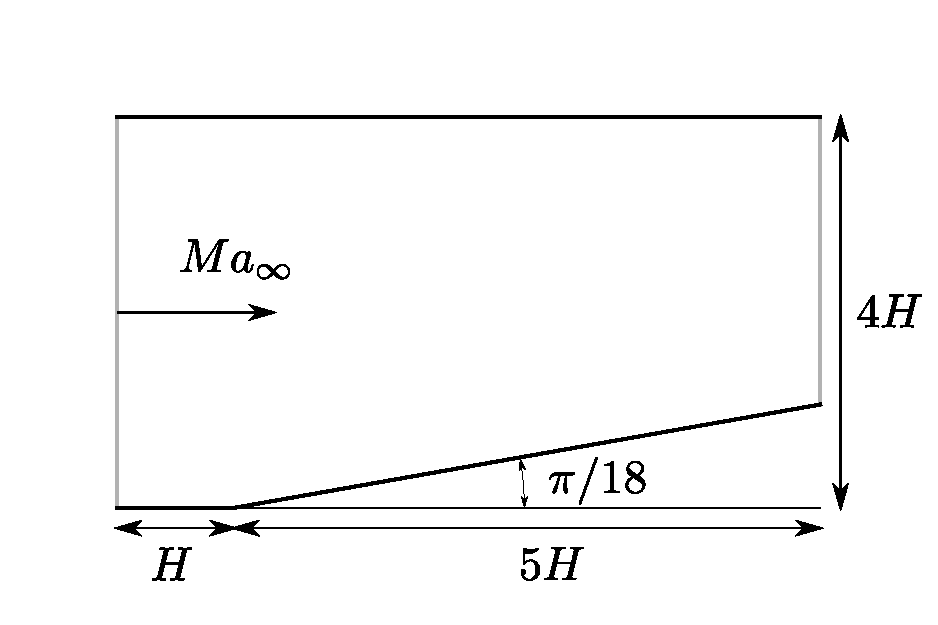
\includegraphics[width=.5\linewidth]{figure/sketch/ramp.pdf}
	\caption{\label{fig:ramp}压缩拐角}
\end{figure}

控制方程(二维Euler方程)如下:
\begin{align}
	 & \left\{\begin{array}{l}
		\dfrac{\partial\rho}{\partial t}+\dfrac{\partial(\rho u)}{\partial x}+\dfrac{\partial(\rho v)}{\partial y}=0           \\[8pt]
		\dfrac{\partial(\rho u)}{\partial t}+\dfrac{\partial(\rho u^2+p)}{\partial x}+\dfrac{\partial(\rho u v)}{\partial y}=0 \\[8pt]
		\dfrac{\partial(\rho v)}{\partial t}+\dfrac{\partial(\rho uv)}{\partial x}+\dfrac{\partial(\rho v^2+p)}{\partial y}=0  \\[8pt]
		\dfrac{\partial(\rho E)}{\partial t}+\dfrac{\partial(\rho Eu+pu)}{\partial x}+\dfrac{\partial(\rho Ev+pv)}{\partial y}=0
	\end{array}\right., \label{eqn:euler2}              \\
	 & \quad \rho E=\frac{p}{\gamma-1}+\frac{1}{2}\rho(u^2+v^2),\quad p=\rho R T
\end{align}
来流条件为:$Ma_\infty=3,\ T_\infty=288.16\ \mathrm{K},\ p=101.325\ \mathrm{kPa}$。此外,$H=10\ \mathrm{m}$,气体参数$R=287\ \mathrm{J/(kg\cdot K)},\ \gamma=1.4$。

\subsection{Coordinate transformation}

\subsection{Dimensional splitting}

\subsection{Numerical methods}

\subsection{Results and discussion}

\newpage
\bibliographystyle{unsrtnat}
\bibliography{ref}

\end{document}